\documentclass{article}
\usepackage[T1]{fontenc}
\usepackage{verbatim}
\usepackage{booktabs}
\usepackage{float}
\usepackage{amsfonts}
\usepackage{amssymb}
\usepackage{amsmath}
\usepackage[table]{xcolor} 
\usepackage{colortbl}
\usepackage{graphicx}
\usepackage{adjustbox}
\usepackage{tabularx}
\usepackage{pgf}
\usepackage{tikz}
\usepackage{placeins}
\usepackage{pgfplots}
\usepackage{pifont}
\usepackage{longtable}
\usepackage[hidelinks]{hyperref}
\title{DINO-Infused Deformable SLAM for Robotic Surgery}
\author{Benjamin Wright}
\date{July 2026}

\begin{document}

\maketitle
\begin{abstract}
Robotic surgery is moving towards higher levels of autonomy, which will require machines to understand the surgical scene in real time: where the endoscope is, what anatomy is present, and how it deforms under interaction. Simultaneous Localisation and Mapping (SLAM) addresses the joint problem of building a map and localising within it, but modern dense neural SLAM systems assume a static world and optimise the camera pose against the map's own predictions, an assumption that fails in surgery, where the scene is itself in motion. Progress is further constrained by data: existing cholecystectomy datasets provide either dense semantic labels or camera-pose ground truth, but not both, and so cannot supervise or evaluate a tracker in a deforming scene.

This thesis addresses both gaps. First, it reorganises the Comprehensive Robotic Cholecystectomy Dataset into a set of self-contained sequences that load under the TUM and Replica conventions, adding dense per-frame semantics from a human-in-the-loop SAM~3 pipeline, stereo-anchored MoGe-2 depth, and cleaned camera trajectories --- establishing, to our knowledge, the only densely-labelled cholecystectomy benchmark with camera-pose ground truth suitable for SLAM evaluation. Second, it presents DID-SLAM, an extension of the deformable neural-SDF system DDS-SLAM with two mechanisms: a learned aleatoric uncertainty that down-weights measurements the static map cannot explain, and a label-free motion attribution that separates camera ego-motion from independent scene motion and freezes the pose when the camera is still. Calibrated on two design sequences and evaluated unseen on three held-out ones, DID-SLAM lowers absolute trajectory error on all five ($-31\%$ on average, $-42\%$ on the largest-travel held-out sequence) at rendering quality that trades $0.6$\,dB of PSNR (the price of a Charbonnier photometric loss that declines to chase specular outliers) for improved SSIM and LPIPS on every sequence, and records the best trajectory of six benchmarked systems on every sequence, the closest contest decided by $0.14$\,mm against a dedicated tracking-only method. The results indicate that on deforming, monocular-depth surgical scenes, a neural-SDF substrate with explicit motion handling tracks more reliably than either render-loss or splatting alternatives.
\end{abstract}

\newpage
\tableofcontents
\newpage

\section*{Notation}
\addcontentsline{toc}{section}{Notation}
Symbols are grouped by the section that introduces them. A few letters are reused
across sections in their own conventional sense; where that happens both meanings
are listed.

\renewcommand{\arraystretch}{1.25}
\begin{longtable}{@{}p{0.24\textwidth} p{0.70\textwidth}@{}}
\toprule
\textbf{Symbol} & \textbf{Meaning} \\
\midrule
\endfirsthead
\toprule
\textbf{Symbol} & \textbf{Meaning} \\
\midrule
\endhead
\bottomrule
\endfoot

\multicolumn{2}{@{}l}{\textit{Neural field and volume rendering (Sections~\ref{sec:coslam})}}\\
$x \in \mathbb{R}^3$ & 3-D query point \\
$d$ & viewing direction (NeRF) \\
$r(z) = o + z\,d$ & camera ray with centre $o$ and depth $z$ along the ray \\
$F_\theta$ & NeRF neural field \\
$\sigma$ & volume density (NeRF only; distinct from the uncertainty variance $\sigma^2$) \\
$c$ & view-independent colour / radiance (distinct from the depth pre-scale $c$ in Depth-$L_1$) \\
$s(x)$ & truncated signed distance from $x$ to the nearest surface \\
$\tau$ & SDF truncation width \\
$h$ & geometry feature returned by the geometry decoder \\
$\gamma_{\text{hash}},\ \gamma_{\text{ob}},\ \gamma$ & multiresolution-hash, one-blob, and joint (concatenated) encodings \\
$g_\theta,\ f_\theta$ & geometry decoder, colour decoder \\
$w_i,\ T_i,\ \delta_i$ & rendering weight, accumulated transmittance, inter-sample spacing at ray sample $i$ \\
$W$ & along-ray normaliser of the SDF rendering weights \\
$\mathrm{S}$ & logistic sigmoid \\
$\hat{C}(r),\ \hat{D}(r)$ & rendered colour and depth of ray $r$ \\
$D,\ z$ & measured depth, and along-ray sample depth (SDF losses) \\
$T,\ F$ & near-surface and free-space sample sets in $\mathcal{L}_{\text{sdf}},\mathcal{L}_{\text{fs}}$ (set-valued; distinct from $T_i$ and $F_\theta$ above) \\
$\lambda_{\text{rgb}},\lambda_d,\lambda_{\text{sdf}},\lambda_{\text{fs}}$ & Co-SLAM loss weights \\
$T_i^{\text{init}}$ & constant-velocity pose initialisation of frame $i$ \\
\midrule
\multicolumn{2}{@{}l}{\textit{Deformation warp (Section~\ref{sec:ddsslam})}}\\
$D_\phi$ & time-conditioned deformation network \\
$\Delta x,\ x_{\text{canon}}$ & displacement to canonical space, and the canonical point $x + \Delta x$ \\
$\gamma_{\text{freq}},\ M$ & frequency (positional) encoding, and its number of bands \\
\midrule
\multicolumn{2}{@{}l}{\textit{Uncertainty-aware down-weighting (Section~\ref{sec:uncertainty})}}\\
$\sigma^2(r)$ & learned per-ray aleatoric variance \\
$\mathcal{L}_{\text{NLL}}$ & heteroscedastic negative log-likelihood \\
$w(r)$ & per-ray tracking trust weight $1/\sigma^2(r)$ \\
$w_{\min},w_{\max}$ & clamp bounds on $w(r)$ \\
$\bar{w}$ & mean weight, used for mean-normalisation \\
\midrule
\multicolumn{2}{@{}l}{\textit{Motion attribution (Section~\ref{sec:motion})}}\\
$K,\ k$ & number of semantic districts, and district index \\
$\delta$ & reference-frame stride for optical flow \\
$f_k,\ Z_k,\ p_k$ & district $k$'s median flow, median depth, and centroid \\
$Z_{\text{med}}$ & median district depth over the frame \\
$\zeta_k = Z_{\text{med}}/Z_k$ & dimensionless depth ratio (cancels the unknown monocular scale) \\
$r_k$ & normalised radial position of district $k$ \\
$p_0,\ r_{\text{norm}}$ & image principal point, and a normalising radius \\
$u,\ v,\ d$ & egomotion coefficients: rotation (depth-blind), lateral slide, radial zoom \\
$\hat{f}_k$ & flow predicted for district $k$ by the egomotion fit \eqref{eq:vote-fit} \\
$\rho_k$ & fit residual $\lVert f_k - \hat{f}_k \rVert$ \\
$w_k$ & district trust weight \\
$\mathrm{med},\ \mathrm{scale}$ & robust centre and spread of the residuals $\{\rho_k\}$ (median and scaled median-absolute-deviation) used in the reweighting \\
$q_{10},\ \tau_q$ & tenth-percentile district flow magnitude (minority test) and its freeze threshold \\
$\mathrm{dis3},\ \tau_d$ & fraction of districts epipolar-inconsistent (majority test) and its freeze threshold \\
$F$ & fundamental matrix fit to the dense flow (distinct from the free-space set $F$ above) \\
\midrule
\multicolumn{2}{@{}l}{\textit{Evaluation metrics (Section~\ref{sec:eval_metrics})}}\\
$\mathbf{x}_i,\ \mathbf{y}_i$ & estimated and ground-truth camera centres, paired by frame \\
$s,\ R,\ \mathbf{t}$ & Sim(3) scale, rotation, translation (Umeyama alignment) \\
$e_i,\ \mathrm{ATE}_{\mathrm{RMSE}}$ & per-frame alignment error, and its root-mean-square \\
$\rho_{\mathrm{path}},\ L(\cdot)$ & scale-corrected path-length ratio, and trajectory arc length \\
$|r|$ & absolute Pearson correlation along the dominant axis (distinct from the ray $r$) \\
$\mu,\ \sigma_{12},\ C_1,\ C_2$ & local mean, cross-covariance, and stabilising constants (SSIM) \\
$\phi_l,\ w_l$ & pretrained deep features and layer weights (LPIPS) \\
$\Omega$ & set of image pixels \\
$\mathcal{V},\ c$ & valid-pixel set and per-model depth pre-scale (Depth-$L_1$) \\
$\mathrm{IoU}_c,\ \mathrm{mIoU}$ & per-class and mean intersection-over-union \\
\end{longtable}
\renewcommand{\arraystretch}{1.0}
\newpage

\section{Introduction}
Robotic surgery is increasingly prevalent, with systems such as the da Vinci surgical robot now used in hospitals worldwide. Yet such systems remain fully tele-operated: the surgeon must maintain continuous spatial awareness of the operating environment through a narrow endoscopic view, with no autonomous element. As the field moves towards higher robotic autonomy, machines will require the understanding the surgeon currently provides: where the camera is, what anatomical structures are present, and how they move under physiological motion and instrument interaction.

The first two requirements form the classical problem of Simultaneous Localisation and Mapping (SLAM): building a map of an unknown environment while localising within it. The two halves are mutually dependent, a chicken-and-egg problem. Modern dense neural SLAM systems such as iMAP~\cite{Sucar2021}, NICE-SLAM~\cite{Zhu2022}, and Co-SLAM~\cite{Wang2023} resolve this through frame-to-model tracking, optimising the camera pose directly against the photometric and geometric predictions of the map itself.

Frame-to-model tracking assumes the map is a fixed, trustworthy reference. In surgery this breaks: the scene itself deforms, so a disagreement between the current frame and the map is ambiguous, indicating either camera motion or tissue motion, and the optimiser cannot distinguish the two. Surgical deformation is also harder than the classical dynamic-scene problem, where discrete moving objects can be detected and masked out~\cite{Bescos2018}; here the deforming content is the anatomy being mapped, and cannot be excised or ignored. A surgical SLAM system must therefore decide, frame by frame, which image motion belongs to the camera and which to the scene (Figure~\ref{fig:problem}). Current systems make this decision only implicitly.

\begin{figure}[!ht]
    \centering
    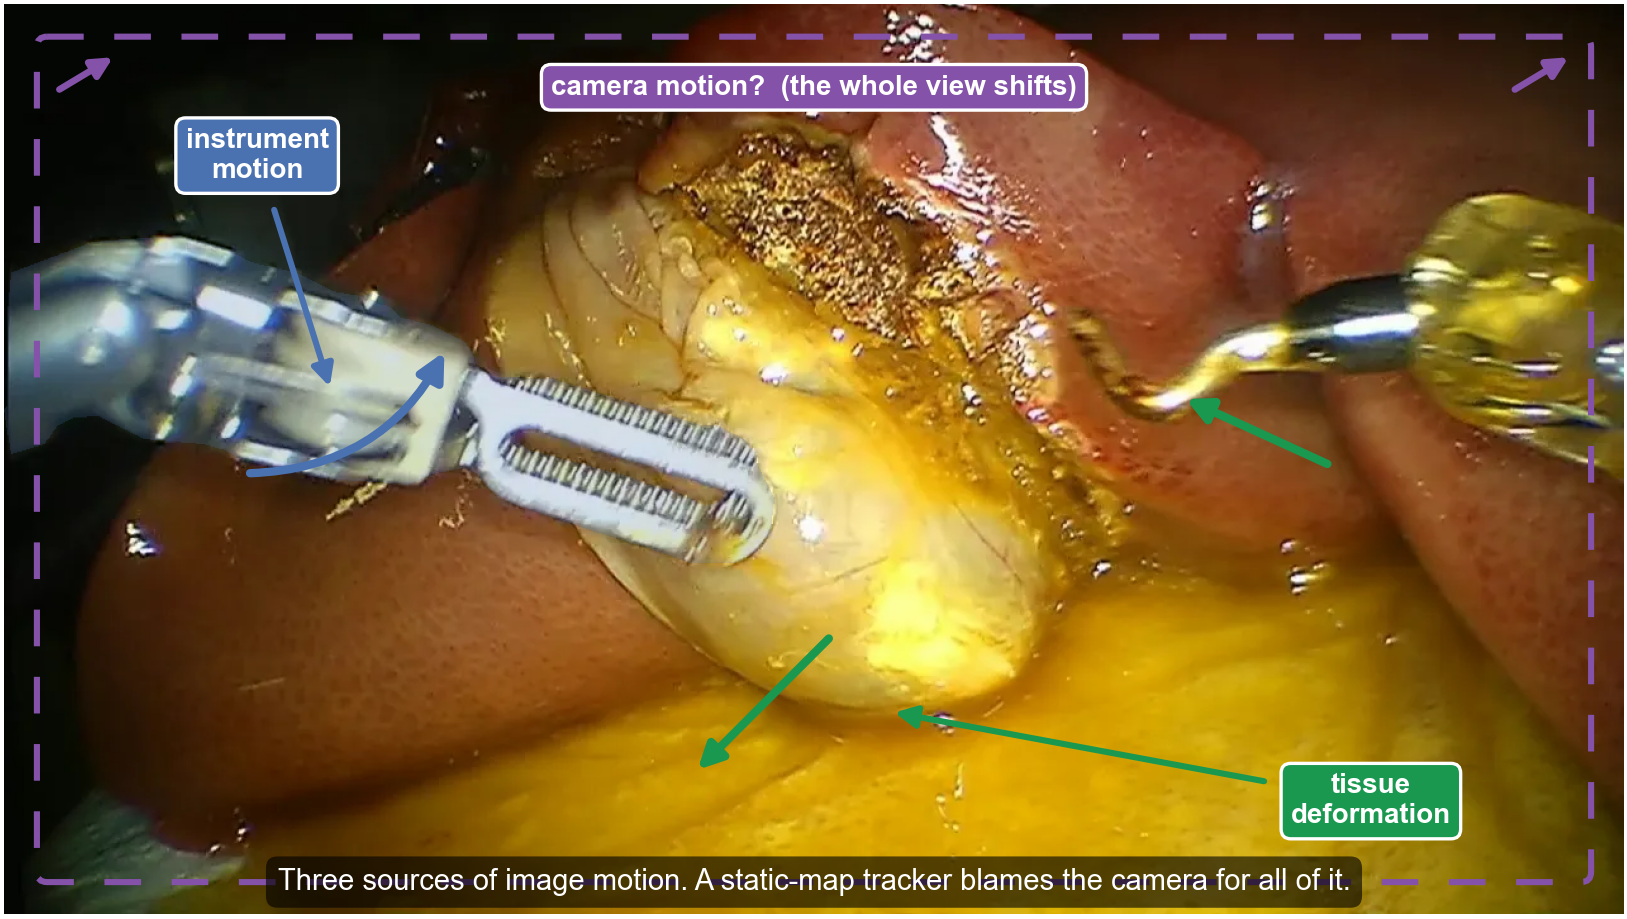
\includegraphics[width=\linewidth]{figures/problem_figure.png}
    \caption{The problem this thesis addresses. In a single surgical frame, an instrument (blue), the tissue it deforms (green), and the camera itself all produce image motion; frame-to-model tracking cannot tell them apart and attributes the disagreement to the camera pose. Frame from C\_2/001; annotations placed from the semantic mask.}
    \label{fig:problem}
\end{figure}
\FloatBarrier

Progress is further constrained by data. To supervise or evaluate a tracker in a deforming scene, a dataset must provide dense semantic labels and camera-pose ground truth simultaneously; existing cholecystectomy datasets provide one or the other. Semantic-SuPer~\cite{Lin2023} carries dense labels but no ground-truth camera poses, and StereoMIS~\cite{Hayoz2023} segments only instruments. The Comprehensive Robotic Cholecystectomy Dataset (CRCD)~\cite{Oh2024} records stereo endoscopic video with synchronised robot kinematics, hence a true camera trajectory, but lacks the dense semantics, metric depth, and benchmark structure a semantic SLAM pipeline requires.

This thesis addresses both gaps. It expands the CRCD into a benchmark on which a tracker can be supervised and honestly evaluated in a deforming scene, and develops a SLAM system that makes the camera-versus-scene decision explicit. The contributions are set out below:

\section{Contributions}
This thesis makes three contributions:
\begin{enumerate}
\item A one-shot, human-in-the-loop segmentation strategy for unseen surgical domains built on the frozen foundation model SAM~3~\cite{Carion2025}: sparse human-annotated anchor keyframes seed SAM~3's video propagation to generate the dense per-frame semantic annotations a semantic SLAM pipeline requires, without fine-tuning.
\item A reorganisation of the CRCD~\cite{Oh2024} into self-contained \texttt{Sequences} consumable by both TUM and Replica data-loaders (Section~\ref{sec:data_packs}), establishing a benchmark for semantic SLAM in surgical environments.
\item \textbf{DID-SLAM} (DINO-Infused DDS-SLAM), an uncertainty-aware extension of DDS-SLAM~\cite{Shan2024} on a neural-SDF substrate (Figure~\ref{fig:did_arch}), contributing: (i) aleatoric-uncertainty down-weighting, ported from WildGS-SLAM~\cite{Zheng2024} to a surgical neural-SDF system via a small uncertainty head (UncertaintyNet) that drives both tracking and mapping; (ii) a label-free split of camera ego-motion from independent scene motion, combining frozen self-supervised vision-transformer features~\cite{Oquab2023,Simoni2025} with a depth-signature egomotion fit and a geometric epipolar agreement, with no trained segmenter --- consumed as a pose freeze that is re-pinned through bundle adjustment so the decision persists in the trajectory. Design choices were locked on two design sequences and evaluated unseen on three held-out ones; the combination improves tracking on all five ($-31\%$ ATE against the unmodified base, $-42\%$ on the largest-travel held-out sequence) while improving SSIM and LPIPS on every sequence, at a cost of $0.6$\,dB of PSNR attributable to the Charbonnier photometric loss.
\end{enumerate}

\begin{figure}[!ht]
    \centering
    \includegraphics[width=\linewidth]{figures/fig_did_slam_overview.png}
    \caption{DID-SLAM: the DDS-SLAM neural-SDF base (grey) extended with two flag-gated contributions (blue) --- a learned uncertainty head and a label-free motion-attribution gate --- with the base left bit-identical when the flags are off.}
    \label{fig:did_arch}
\end{figure}
\FloatBarrier


\section{Related Works}
\paragraph{Classical and deformable SLAM.}
ORB-SLAM3~\cite{Campos2021} exemplifies classical feature-based (sparse) SLAM, unifying multi-map data association across monocular, stereo, and RGB-D inputs. While accurate, such indirect methods assume a rigid scene, an assumption violated by moving objects in a dynamic environment. DefSLAM~\cite{Lamarca2020} introduced real-time monocular SLAM for deforming scenes, combining Shape-from-Template tracking with isometric Non-Rigid Structure-from-Motion for map updates. Its successor SD-DefSLAM~\cite{Rodrguez2020} improved robustness in surgical environments by fusing direct and indirect data association and using CNN-based semantic segmentation to mask surgical tools, demonstrating the value of semantics for handling dynamic objects that would otherwise corrupt tracking and mapping.

\paragraph{Neural-implicit SLAM.}
iMAP~\cite{Sucar2021} used a single MLP as a unified scene representation for real-time joint tracking and mapping; NICE-SLAM~\cite{Zhu2022} introduced hierarchical feature grids; and Co-SLAM~\cite{Wang2023} combined a multi-resolution hash grid with one-blob coordinate encodings for robust tracking and smooth reconstruction. These systems optimise the camera pose against the map's own photometric and geometric predictions (frame-to-model tracking). All assume a static world, relying on trust in the map for accurate pose updates.

\paragraph{Dense optical-flow tracking.}
A separate lineage estimates the camera from dense correspondence rather than a map's own predictions. DROID-SLAM~\cite{Teed2022} couples recurrent optical-flow updates with a dense bundle-adjustment layer, achieving strong tracking accuracy on both indoor and driving benchmarks; its endoscopic adaptation (evaluated later as PERSEUS) is the tracking-only reference in this thesis. Solving only for pose from flow, such systems carry no scene representation to render or to reason about deformation; and the flow-gating heuristic that suppresses sub-threshold motion, needed to avoid drift on near-static video, is precisely what makes them stop updating when true motion falls below the flow noise floor.

\paragraph{Neural scene representations in surgery.}
The shift towards dense scene representations in surgery began in parallel, with EndoNeRF~\cite{Wang2022} applying neural radiance fields in a canonical-plus-deformation framework to reconstruct deforming tissue under tool interaction. However, EndoNeRF and its successors assume known camera poses and do not address joint localisation and mapping. More recently, Gaussian-splatting representations have been adopted for surgical SLAM: EndoGSLAM~\cite{Wang2024} demonstrated dense reconstruction at over 100 frames per second using differentiable Gaussian rasterisation, though under a rigid-scene assumption and requiring RGB-D input.

\paragraph{Robustness to dynamic content.}
Handling scene content that moves independently of the camera is a long-standing SLAM problem with two dominant strategies. Mask-based methods such as DynaSLAM~\cite{Bescos2018} detect movable objects with a trained segmenter and excise them from tracking; effective where reliable detectors exist, but dependent on supervised class knowledge that is scarce in surgery. Uncertainty-based methods instead learn where the data is unreliable: NeRF On-the-go~\cite{Ren2024} trains a shallow MLP on DINOv2 features~\cite{Oquab2023} to predict a per-pixel uncertainty that removes transient distractors from in-the-wild NeRF reconstruction, and WildGS-SLAM~\cite{Zheng2024} carries the same design into Gaussian-splatting SLAM, down-weighting both tracking and mapping without explicit masks. In endoscopy, Hayoz et al.~\cite{Hayoz2023} learn per-pixel weights that robustify camera-pose estimation against tool, specularity and deformation pixels, the closest surgical antecedent of the down-weighting developed here. This thesis ports this second strategy, via the heteroscedastic loss of Kendall and Gal~\cite{KendallGal2017}, onto a neural-SDF surgical substrate, and pursues the label-free goal by geometric rather than learned means.

\paragraph{Semantic surgical perception and DDS-SLAM.}
Semantic-SuPer~\cite{Lin2023} demonstrated that integrating semantics with geometric tracking improves data association and reconstruction in deforming endoscopic scenes. Building on this, DDS-SLAM~\cite{Shan2024} introduced a dense deformable semantic neural SLAM for endoscopy, extending the Co-SLAM substrate with an MLP-based 4D deformation field and a semantic distance-field loss that exploits inter-category boundaries to guide optimisation, reporting improved tracking and reconstruction over both rigid neural-SLAM baselines and prior deformable methods. This work builds upon DDS-SLAM and applies it to the CRCD, integrating foundation-model segmentation with deformable neural SLAM for surgical scene understanding.
\section{Dataset}
The Comprehensive Robotic Cholecystectomy Dataset (CRCD)\cite{Oh2024} records cholecystectomy procedures on pig livers using a first-generation da Vinci surgical system controlled through the da Vinci Research Kit (dVRK), capturing two of the three Patient Side Manipulators (PSMs) and the Endoscope Camera Manipulator (ECM). Seven surgeons (A--G) each performed the procedure one to three times, for 18 episodes in total.

The dataset spans approximately 75 GB across 164 synchronised Parquet files:

\begin{enumerate}
    \item \textbf{Stereo endoscopic video} at $1280 \times 720$ resolution (AVC1/MP4) with embedded ROS timestamps, nominally 60\,fps (episodes A\_1, E\_1, E\_2, and E\_3 at $\sim$54.55\,Hz).
    \item \textbf{Full robot kinematics} comprising PSM1/2 and MTMR/L joint states, Cartesian poses, gripper angles, and the ECM pose as a 7-dimensional vector $(t_x, t_y, t_z, q_x, q_y, q_z, q_w)$, the ground truth camera trajectory for SLAM evaluation.
    \item \textbf{Binary pedal signals} (camera, clutch, monopolar, bipolar) interpolated to the kinematic sampling rate.
\end{enumerate}
\subsection{Dataset Analysis}
Table~\ref{tab:dataset_overview} summarises per-episode motion statistics from the automated motion analysis pipeline of Section~\ref{sec:motion_analysis}. The camera is stationary for 97--99\% of frames across all episodes; only 199 motion segments were identified, comprising 26{,}289 frames and approximately 7.4\,minutes of camera motion at 60~FPS.
\begin{table}[!ht]
\centering
\caption{Per-episode motion summary for all 18 CRCD episodes. \textit{Segs}: number of extracted motion segments; \textit{Mot.\ Fr.}: total motion frames; \textit{Mot.\ (s)}: total motion duration; \textit{Max $v_\text{lin}$} and \textit{Max $\omega$}: peak linear (mm/s) and angular ($^\circ$/s) velocities; \textit{Path}: cumulative camera path (mm); \textit{Rot}: cumulative rotation ($^\circ$);}
\label{tab:dataset_overview}
\resizebox{\textwidth}{!}{%
\begin{tabular}{lrrrrrrrc}
\toprule
\textbf{Episode} & \textbf{Segs} & \textbf{Mot.\ Fr.} & \textbf{Mot.\ (s)} &
\textbf{Max $v_\text{lin}$} & \textbf{Max $\omega$} &
\textbf{Path (mm)} & \textbf{Rot ($^\circ$)} \\
\midrule
A\_1 &  4 &    305 &   5.5 &  26.0 &  30.4 &   39.0 &   41.8 & \\
\midrule
B\_1 &  5 &    513 &   8.5 &  29.7 &  24.6 &   70.2 &   31.9 & \\
B\_2 &  7 &  1{,}023 &  16.9 &  44.1 &  32.1 &  124.8 &   83.5 & \\
B\_3 &  8 &    533 &   8.9 &  63.9 &  22.4 &  109.1 &   51.5 & \\
\midrule
C\_1 &  3 &    340 &   6.7 &  18.0 &  17.4 &   41.2 &   32.6 & \\
C\_2 &  8 &  1{,}192 &  19.7 &  49.2 &  43.8 &  156.9 &  122.4 & \\
C\_3 & 18 &  1{,}752 &  29.3 & 103.4 &  47.3 &  325.8 &  207.8 & \\
\midrule
D\_2 & 12 &  1{,}420 &  23.5 &  48.8 &  20.6 &  218.0 &  109.8 & \\
D\_3 & 12 &    988 &  17.0 &  70.3 &  30.3 &  253.3 &  116.8 & \\
\midrule
E\_1 & 15 &  1{,}651 &  30.0 & 324.0 & 135.8 &  311.2 &  146.5 & \\
E\_2 &  8 &  1{,}114 &  20.3 & 170.2 &  65.4 &  170.4 &   90.1 & \\
E\_3 &  5 &    604 &   11.0 &  86.0 &  35.7 &  150.5 &   79.0 & \\
\midrule
F\_1 & 10 &  3{,}077 &  51.1 &  64.3 &  30.5 &  195.1 &  176.9 & \\
F\_2 &  6 &  1{,}275 &  21.1 &  27.8 &  23.9 &   67.7 &   79.2 & \\
F\_3 &  7 &    898 &  14.9 &  18.6 &  24.8 &   55.0 &   60.2 & \\
\midrule
G\_1 & 13 &  1{,}978 &  32.7 &  25.7 &  11.4 &  146.2 &   63.6 & \\
G\_2 & 37 &  5{,}207 &  86.2 &  23.2 &  15.7 &  386.6 &  240.1 & \\
G\_3 & 21 &  2{,}419 &  40.0 &  14.1 &  18.8 &  135.1 &  130.9 & \\
\bottomrule
\end{tabular}%
}
\end{table}
\FloatBarrier
\subsubsection{Velocity Detection}
\label{sec:motion_analysis}
For each frame, the ECM pose was extracted as a 7-vector $(t_x, t_y, t_z, q_x, q_y, q_z, q_w)$ from the synchronised kinematic stream. Linear velocity was the Euclidean norm of the finite-difference position delta, normalised by the inter-frame interval; angular velocity was derived from the quaternion inner product between consecutive frames:

\begin{equation}
    \omega_i = \frac{2\arccos\left(|\mathbf{q}_i \cdot \mathbf{q}_{i+1}|\right)}{\Delta t_i}
\end{equation}

A frame was classified as containing camera motion when the linear velocity exceeded 0.1\,mm/s or the angular velocity exceeded 0.1\,$^\circ$/s, thresholds chosen empirically to exclude sensor noise while capturing deliberate repositioning. Contiguous motion frames were grouped into segments, discarding bursts shorter than 5 frames to filter residual noise. Because CRCD motion sequences are short, padding extended snippets or concatenated multiple sequences, yielding a range from 200 to just over 2000 frames.

\subsubsection{Scene Motion Classification}
Each segment was further classified by motion type. Tool motion was detected by applying the same finite-difference velocity computation to the PSM1 and PSM2 setpoint Cartesian poses, with a threshold of 1.0\,mm/s (higher than the camera threshold to account for larger expected tool displacements), and each segment labelled \texttt{camera\_only}, \texttt{tool\_only}, or \texttt{tool\_and\_camera}. Tissue motion was classified by manual review, and scripting extracted all segments suitable for SLAM pipelines.

\subsubsection{Selected Sequences}
Sequences were selected for variety in length, motion, and deformation, giving a balanced, challenging surgical SLAM dataset reflective of a real surgical environment. The final published dataset comprises 20 snippets drawn from 10 episodes (B\_2, C\_1, C\_2, C\_3, E\_1, E\_3, F\_1, F\_3, G\_2, G\_3), totalling 14{,}688 stereo frame pairs (Table~\ref{tab:motion}). Camera metrics are computed from the published per-snippet \texttt{groundtruth.txt} (ECM pose per frame); tool paths from the CRCD dVRK kinematics over the matching frame range. A frame counts as a motion frame when inter-frame camera velocity exceeds 0.5\,mm/s (linear) or 1$^\circ$/s (angular); mean velocities are over motion frames only. These trajectories can be visualised using evo~\cite{grupp2017evo}:

\begin{figure}[!ht]
    \centering
    \includegraphics[width=\linewidth]{figures/evo_trajectories.png}
    \caption{Ground-truth camera trajectories of 3 of the 20 published snippets, rendered with \texttt{evo}~\cite{grupp2017evo}. Each curve is the ECM-tip path over its snippet, coloured by normalised time; together they span the range of motion magnitudes and regimes summarised in Table~\ref{tab:motion}.}
    \label{fig:evo_trajectories}
\end{figure}
\FloatBarrier
The full list of sequences is provided in Table~\ref{tab:motion}.
\begin{table}[ht]
\centering
\caption{Published snippet motion statistics. Velocities in mm/s (linear) and $^\circ$/s (angular); paths in mm. Durations cover the full published snippet (including stationary durations).}
\label{tab:motion}
\resizebox{\textwidth}{!}{%
\begin{tabular}{llrrrrrrrrrr}
\hline
\textbf{Ep.} & \textbf{\#} & \textbf{Frames} & \textbf{Dur (s)} & \textbf{Mot. Fr.} &
\textbf{Path} & \textbf{Disp.} & \textbf{Rot ($^\circ$)} &
\textbf{$\bar{v}_\text{lin}$} & \textbf{$\bar{v}_\text{ang}$} &
\textbf{PSM1 Path} & \textbf{PSM2 Path} \\
\hline
B\_2 & 001 & 1321 & 22.00 & 285 & 37.79 &  5.60 & 41.2 &  7.96 &  8.67 & 298.12 &  62.80 \\
\hline
C\_1 & 001 &  360 &  5.98 & 143 & 18.55 & 17.62 & 10.6 &  7.77 &  4.24 &  36.03 &  70.60 \\
\hline
C\_2 & 001 &  730 & 12.15 & 338 & 56.28 & 32.53 & 53.0 &  9.99 &  9.19 & 169.59 & 236.78 \\
\hline
C\_3 & 001 & 1527 & 25.81 & 390 & 78.79 & 30.98 & 53.7 & 11.94 &  8.11 & 283.48 & 339.72 \\
\hline
E\_1 & 001 & 2108 & 38.63 & 361 & 85.88 & 42.45 & 50.0 & 12.97 &  7.49 & 792.17 & 629.81 \\
\hline
E\_3 & 001 &  480 &  8.78 & 173 & 52.80 & 29.35 & 28.2 & 16.65 &  8.69 & 129.00 & 178.14 \\
E\_3 & 002 &  278 &  5.08 &  91 & 23.56 &  5.27 & 15.8 & 14.12 &  9.34 &  63.70 &  46.69 \\
E\_3 & 003 &  263 &  4.80 &  29 & 13.30 &  4.16 &  6.8 & 25.01 & 11.25 &  69.87 &  57.72 \\
E\_3 & 004 &  360 &  6.58 &  98 & 32.91 & 10.01 & 15.6 & 18.32 &  8.29 & 104.61 &  94.83 \\
E\_3 & 005 &  265 &  4.84 & 135 & 43.45 &  9.32 & 19.6 & 17.55 &  7.81 &  76.64 &  60.13 \\
\hline
F\_1 & 002 & 1287 & 21.43 & 473 & 45.20 &  6.95 & 54.5 &  5.73 &  6.79 & 229.84 & 240.56 \\
\hline
F\_3 & 001 &  602 & 10.02 & 148 & 11.83 &  5.48 &  8.4 &  4.79 &  2.89 & 101.05 &  47.25 \\
F\_3 & 002 &  312 &  5.18 &  66 &  6.67 &  4.74 &  7.2 &  6.05 &  6.36 &  78.87 &  35.51 \\
F\_3 & 003 &  400 &  6.65 &  72 &  4.18 &  3.20 &  5.9 &  3.48 &  4.19 &  85.15 &  59.69 \\
F\_3 & 004 &  200 &  3.32 &  62 &  9.44 &  8.50 & 12.8 &  9.14 & 12.32 &  64.16 &  66.22 \\
F\_3 & 005 &  200 &  3.32 &  70 &  7.73 &  6.60 & 10.3 &  6.62 &  8.85 &  22.58 &  17.52 \\
F\_3 & 006 &  387 &  6.45 & 108 &  8.90 &  3.98 &  9.3 &  4.94 &  5.02 &  44.36 &  31.64 \\
F\_3 & 007 &  300 &  4.98 &  89 &  6.57 &  2.77 &  9.2 &  4.43 &  6.12 &  57.60 &  28.88 \\
\hline
G\_2 & 003 & 1321 & 22.00 & 257 & 35.02 & 18.68 & 18.8 &  8.18 &  4.17 & 204.13 & 176.27 \\
\hline
G\_3 & 001 & 1987 & 33.10 & 353 & 31.57 & 23.09 & 26.2 &  5.36 &  4.14 & 232.35 & 320.52 \\
\hline
\end{tabular}%
}
\end{table}
\FloatBarrier
\subsubsection{Comparison with existing segmentation datasets}
\label{sec:dataset_comparison}
When comparing the aforementioned to existing cholecystectomy datasets, five such others exist --- CholecSeg8k~\cite{Hong2020}, CholecInstanceSeg~\cite{Alabi2025}, Endoscapes2023~\cite{Murali2024}, CRCD (Expanded)~\cite{Oh2024}, and HeiSurF/HeiChole~\cite{Wagner2023} --- and they differ along axes that matter directly for deformable surgical SLAM: subject (in-vivo human versus ex-vivo porcine), imaging modality (monocular versus stereo), the availability of camera-pose ground truth, and whether the sliding-interface event central to this thesis, the separation of the gallbladder from the liver bed, is captured at all. Table~\ref{tab:dataset_comparison} summarises the comparison.

\begin{table}[!ht]
\centering
\caption{Public pixel-level segmentation datasets for laparoscopic cholecystectomy. Annotated frame counts cite the annotated portion only, not the raw video corpus. CRCD is the only stereo dataset with camera-pose and kinematic ground truth, at annotation scale comparable to CholecSeg8k.}
\label{tab:dataset_comparison}
\footnotesize
\setlength{\tabcolsep}{3pt}
\begin{tabular}{l r c c l}
\toprule
\textbf{Dataset} & \textbf{Frames} & \textbf{Pose} & \textbf{Stereo} & \textbf{Semantics} \\
\midrule
CholecSeg8k        & 8{,}080         & \ding{55} & \ding{55} & Tool+tissue; 13 cls (manual) \\
CholecInstanceSeg  & $\sim$30{,}000  & \ding{55} & \ding{55} & Tool inst.; tissue only on CS8k base \\
Endoscapes2023     & 493             & \ding{55} & \ding{55} & Tool+tissue; 6 cls (Seg50, manual) \\
HeiSurF/HeiChole   & sparse          & \ding{55} & \ding{55} & Tool+tissue; 21 cls (manual) \\
\textbf{Ours (exp. CRCD)} & \textbf{14{,}688} & \ding{51} & \ding{51} & Tool+tissue; 4 cls (SAM3, HITL) \\
\bottomrule
\end{tabular}
\end{table}

Of these, CholecInstanceSeg is tool-instance only on its $\sim$30{,}000-frame CholecT50-full bulk; its anatomy labels are inherited from the CholecSeg8k base, so for tool-plus-tissue segmentation it effectively collapses to CholecSeg8k. Endoscapes2023 is phase-restricted and excludes the gallbladder-from-liver-bed separation (a major deforming event in the procedure), releasing only 493 public segmentation masks. HeiSurF carries the richest taxonomy (21 full-scene classes) but samples sparsely at two-minute intervals. CholecSeg8k and CRCD are therefore the two datasets that combine dense tool-and-tissue segmentation with full-procedure coverage; CholecSeg8k, however, is limited to 80-frame clips, too short for full SLAM evaluations (when compared to the 200--2000 frame sequences we provide).

 CholecSeg8k provides manual tissue masks on real in-vivo human cholecystectomy; its limitation is that it is monocular and carries no camera-pose ground truth, so it cannot supervise or evaluate a tracker; additionally, the short sequence length makes the dataset unsuitable for SLAM. CRCD supplies rectified stereo pairs enabling metric depth recovery, per-frame ECM camera pose and dVRK kinematics giving trajectory ground truth. Its costs are that the tissue masks are SAM3 propagations from sparse human labels which are then fine-tuned by a human annotator. Additionally, the ex-vivo porcine setting removes respiratory motion present in the in-vivo human datasets. For a deformable SLAM system that requires camera-pose ground truth to evaluate tracking, CRCD is the only one of the five that provides it, making it the only densely semantically labelled cholecystectomy dataset suitable for SLAM evaluation.
\subsection{Semantic Annotations}

The expanded CRCD \cite{Oh2024} provides COCO-format annotations for liver segmentation and instrument keypoint detection. Three recordings (C\_1, E\_3, F\_3) include human-annotated ground truth masks at every 120th frame, the reference for the one-shot segmentation experiments. These sparse annotations are propagated to the remaining 119 frames of each 120-frame \texttt{split} by a Track Anything model~\cite{Yang2023}. The release also includes surgeon experience profiles (number and complexity of prior laparoscopic procedures, hours of robotic training).

This coverage is limited for deformable-scene SLAM: only three of the eighteen episodes (C\_1, E\_3, F\_3) carry any segmentation reference.

We therefore expand this into a dense, per-frame semantic segmentation dataset covering all 20 published snippets: 14{,}688 annotated left-camera frames, each with its rectified right-camera counterpart, labelled under one of three classes --- Liver, Gallbladder, and Tool --- chosen as reliably annotatable and relevant to the downstream SLAM task. Masks are produced with a SAM~3-in-the-loop pipeline: a small set of human-painted anchor keyframes per snippet is propagated bidirectionally through the clip by the SAM~3 video predictor, then inspected; failure frames are corrected and re-committed as additional anchors, and the clip is re-propagated until per-frame quality is reached. The masks ship in every data package as the dense \texttt{semantic\_instance/} rasters and COCO \texttt{snippet\_annotations.json} of Section~\ref{sec:data_packs}; the full pipeline appears in Section~\ref{sec:segmentation}.
\subsubsection{SAM~3}
Segment Anything Model 3 (SAM~3)~\cite{Carion2025} is a foundation model for promptable segmentation extending SAM~\cite{Kirillov2023} and SAM~2~\cite{Ravi2024}. Where prior SAM models used geometric prompts (points, boxes, masks), SAM~3 adds \textit{Promptable Concept Segmentation} (PCS): concept prompts defined by noun phrases (e.g., ``tools''). These are processed by the text encoder within the shared Perception Encoder backbone, while geometric prompts go to the tracker inherited from SAM~2.
\begin{figure}
    \centering
    \includegraphics[width=1\linewidth]{figures/fig_sam3_architecture.png}
    \caption{SAM~3 architecture: the split between video and text prompting.}
    \label{fig:sam3arch}
\end{figure}
\FloatBarrier

SAM~3 pairs a \textit{detector} and \textit{tracker} sharing a Perception Encoder (PE) backbone~\cite{Bolya2025}. The DETR-based detector~\cite{Carion2020} fuses text/exemplar prompt tokens with image features via cross-attention, then decodes learned object queries into binary classification logits and bounding boxes. A \textit{presence token} decouples recognition from localisation, independently assessing whether a candidate region matches the queried concept, which helps distinguish semantically similar structures (e.g., liver vs.\ gallbladder). The tracker inherits the SAM~2 streaming architecture: a memory module stores prior-frame information, and memory attention conditions each new frame embedding for temporally consistent mask propagation, including through occlusions.
SAM~3 was trained on 4M unique concept labels (52M masks) plus a synthetic set of 38M phrases (1.4B masks), and achieves 75--80\% of human performance on the SA-Co benchmark ($>$207K concepts)~\cite{Carion2025}. Here it is deployed frozen, without medical-domain fine-tuning, on CRCD endoscopic videos. Its text prompting enables concept-level queries (e.g., ``tools'') without geometric prompts, reducing manual annotation dependence relative to SAM~2.
\begin{figure}[!ht]
\centering
    \includegraphics[width=1\linewidth]{figures/annotation_pipeline_ucl.png}
    \caption{SAM~3 architecture as modified for CRCD deployment.}
    \label{fig:SAM3Mod}
\end{figure}
\FloatBarrier
\subsection{Prompting}
\label{sec:prompting}
\subsubsection{Prompting Strategies}
With SAM~3 deployed frozen, the prompting strategy critically determines segmentation quality, and prompt errors compound through temporal propagation. CRCD ground truth masks (every 120 frames for C\_1, E\_3, F\_3) supplied the geometric prompts for liver and gallbladder, but were insufficient for a full SLAM evaluation pipeline. Annotation was therefore expanded to the full CRCD with the following prompting strategies:
\begin{enumerate}
    \item \textbf{Bounding box:} axis-aligned box from the ground truth mask.
    \item \textbf{Positive points:} points sampled within the mask region.
    \item \textbf{Positive + negative points:} positive points within the mask and negative points from background near the object boundary, disambiguating the target from adjacent tissue.
    \item \textbf{Combined:} bounding box, positive, and negative points together, the most information-rich geometric prompt.
    \item \textbf{Text (SAM~3 only):} noun phrase prompts (e.g., ``tools'', ``liver'', ``gallbladder'') with no geometric guidance, testing fully automated segmentation.
    \item \textbf{Masks:} full human annotated masks.
\end{enumerate}
\begin{figure}[!ht]
    \centering
    \includegraphics[width=1\linewidth]{figures/fig_annotator_workflow.pdf}
    \caption{The keyframe annotation workflow. Geometric prompts --- bounding boxes and positive/negative point clicks --- are placed on a keyframe in the browser annotator and issued to SAM~3, which propagates the resulting masks through the clip.}
    \label{fig:PromptingMethods}
\end{figure}
\FloatBarrier

Of the text prompts, only ``tools'' yielded any results, as SAM~3 was not trained on medical data. Prompts were issued at annotated frames and propagated temporally via the model's memory mechanism.

The six strategies gave mixed results on the CRCD. Combined prompting (positive and negative points, bounding boxes, and text prompts for tools) was best among the native SAM~3 strategies, but given the scene complexity and SAM~3's difficulty with medical-domain data, mask-based prompting gave the best results overall.

A result of all 6 annotation methods on a chosen frame is shown in Figure~\ref{fig:PromptingMethodsResults}:
\begin{figure}[!ht]
    \centering
    \includegraphics[width=1\linewidth]{figures/fig_segmentation_6styles.png}
    \caption{Segmentation output of the six prompting strategies --- bounding box, positive points, positive + negative points, combined, text, and full mask --- on a challenging frame. Combined geometric prompting gives the best of the native SAM~3 strategies, while mask-based prompting is the most reliable on this out-of-domain surgical data. Noting that in this randomised example `text' prompting returned no valid masks.}
    \label{fig:PromptingMethodsResults}
\end{figure}
\FloatBarrier
\subsubsection{Annotation Pipeline}
\label{sec:segmentation}
Manual hand-annotation of every frame in the CRCD would be infeasible. Instead, a keyframe-anchored, human-in-the-loop (HITL) pipeline was built around SAM~3's video propagation (Figure~\ref{fig:SAM3Mod}), running on a FastAPI/Konva.js annotator.

Selected frames are assigned as keyframes and hand-annotated in the browser annotator (brush, SAM-click, SAM-box and bucket-fill tools, with per-class erasers). Keyframes were typically placed every 60--120 frames depending on sequence difficulty, with extra keyframes where significant deformation or camera motion occurred or new artefacts entered the scene. For example, CRCD sequence C\_1/001 was given keyframes at frames 0, 119, 239 and 359.

Committed anchor masks seed SAM~3's video predictor, propagated both forwards and backwards from every anchor --- a modification of the as-built SAM~3 pipeline, which propagates forward-only from a single prompt frame. Where the forward and backward sweeps disagree, the mask with the higher SAM~3 confidence score is retained. A drop in confidence, or a sudden change in the pixel count of a taxonomy class (suggestive of a mask dropout, e.g.\ a tool no longer registered), flags the frame for review. Because SAM~3's decoder reconstructs and smooths masks even at prompt frames, the user-painted anchor masks are re-imposed verbatim at their keyframes after propagation, so the human annotation is never silently overwritten. On local hardware, propagation can be deferred entirely: anchors are painted in a lightweight mode (without the model loaded) and propagated later on a rented A100 by replaying the same session file.

The propagated masks are rendered as a mask-overlay video scrubbed end-to-end by the annotator. `Failed' frames are corrected in one of three ways, in increasing order of effort: (i) direct hand-fix in the annotator; (ii) insertion of additional keyframes followed by re-propagation of only the affected window (bounded to the failure region, then stitched back into the accepted sequence); or (iii) full re-anchoring of the sequence. This loop iterates until the annotator accepts the full sequence.

Accepted masks are resolved to a single class per pixel under an occlusion-priority (Tool $>$ Gallbladder $>$ Liver, reflecting physical foreground order; per-frame overrides are supported for sequences where semantic classes overlap), rasterised to per-frame semantic label maps, and passed through a four-gate check (dataset-consistency audit, TUM-loader test, intrinsics sanity check, and byte-stable regeneration). A sequence is published only once all four gates pass \emph{and} the HITL annotator has signed off the final overlay render. These masks and their quality are compared to the provided CRCD annotations in the figure below, with frames randomly selected across the annotated sequences.
\FloatBarrier
\begin{figure}[!ht]
    \centering
    \includegraphics[width=1\linewidth]{figures/fig_annotation_comparison.png}
    \caption{Segmentation output of SAM~3 compared with Track Anything across a range of frames and sequences. \textbf{Ours} shown on the left hand side, \textbf{CRCDs provided} annotations shown on the right}
    \label{fig:PromptingComparison}
\end{figure}
\FloatBarrier
\subsection{Sequences}
\label{sec:data_packs}
\subsubsection{Format}
Each motion segment identified above is packaged into a self-contained \textit{data package}: a directory holding everything required to run and evaluate a SLAM method. To keep the packages consumable without modification by established RGB-D SLAM frameworks, each is laid out to simultaneously satisfy the TUM RGB-D \cite{sturm11rss-rgbd} and Replica \cite{Straub2019} benchmark conventions: the pose stream adopts the TUM trajectory convention, the per-frame semantic masks the Replica \texttt{info\_semantic.json} convention, and a right-camera stream is appended as a backward-compatible stereo extension. Table~\ref{tab:snippet_contents} lists the contents of each package.

\begin{table}[ht]
\centering
\caption{Contents of each data package.}
\label{tab:snippet_contents}
\begin{tabular}{lp{7cm}}
\hline
\textbf{Artefact} & \textbf{Description} \\
\hline
\texttt{rgb/} & Left-camera frames, $1280\times720$ PNG, timestamp-named. \\
\texttt{rgb.txt} & TUM index: one \texttt{timestamp filename} pair per line. \\
\texttt{rgbright/} & Right-camera frames (stereo extension). \\
\texttt{rgbright.txt} & TUM index for the right camera. \\
\texttt{depth/} & Depth PNGs generated by MoGe-2. \\
\texttt{depth.txt} & TUM index retained for loader compatibility. \\
\texttt{associations.txt} & TUM nearest-timestamp associations linking RGB, depth, and pose entries. \\
\texttt{groundtruth.txt} & ECM-tip trajectory in TUM format (\texttt{timestamp tx ty tz qx qy qz qw}). \\
\texttt{intrinsics.yaml} & Rectified $K$ matrix, stereo baseline, rectification parameters. \\
\texttt{info\_semantic.json} & Replica-style class taxonomy; dense 3-class (\texttt{id == coco\_id}, \texttt{pixel\_value == id + 1}). \\
\texttt{semantic\_instance/} & Per-frame semantic rasters, single-channel \texttt{uint16} PNG; pixel value $=$ class id $+\,1$, with 0 for background (i.e., unassigned). \\
\texttt{snippet\_annotations.json} & COCO polygon annotations (Liver, Gallbladder, Tool). \\
\texttt{snippet\_overlay.mp4} & Rendered semantic overlay video. \\
\hline
\end{tabular}
\end{table}

\subsubsection{TUM RGB-D conventions}

Image streams are indexed in the TUM manner: \texttt{rgb.txt} and its right-frame counterpart \texttt{rgbright.txt} list one \texttt{timestamp filename} pair per line, filenames keyed on the ROS timestamp inherited from the synchronised CRCD Parquet files. The ground-truth trajectory is written to \texttt{groundtruth.txt} as \texttt{timestamp $t_x$ $t_y$ $t_z$ $q_x$ $q_y$ $q_z$ $q_w$} records expressing the endoscope (ECM-tip) pose as a position and unit quaternion in a fixed world frame, the representation consumed by the standard TUM \texttt{evaluate\_ate} and \texttt{evaluate\_rpe} tooling. Since every stream derives from the source's synchronised timeline, \texttt{associations.txt} records the nearest-timestamp correspondence between RGB, depth, and pose entries that TUM-style loaders expect.

\subsubsection{Replica semantic conventions}

Semantic ground truth follows the Replica semantic-segmentation convention. \texttt{info\_semantic.json} declares the class taxonomy as an ordered list of \texttt{(id, name)} entries --- here the dense three-class scheme \texttt{\{0:\,Liver, 1:\,Gallbladder, 2:\,Tool\}} --- and per-frame labels are stored in \texttt{semantic\_instance/} as single-channel \texttt{uint16} PNGs. The invariant \texttt{pixel\_value $=$ class\_id $+\,1$} holds throughout, with pixel value 0 reserved for background, so a Replica-style reader recovers the class map directly from the raster while background stays unambiguously non-object. The identical masks are also provided as COCO polygons in \texttt{snippet\_annotations.json} for consumers preferring vector annotations, kept pixel-consistent with the raster by construction. Both forced conventions ease use of the CRCD with SLAM models.

\subsubsection{Stereo, depth, and intrinsics}

Two adaptations carry the monocular benchmark formats to the stereo, depth-free surgical setting. First, the right-camera stream (\texttt{rgbright/}, \texttt{rgbright.txt}) is appended so stereo methods compute disparity directly while monocular readers ignore it. Second, \texttt{intrinsics.yaml} carries a \texttt{depth\_placeholder: true} sentinel signalling that metric depth is derived from the stereo pair rather than read from disk; the directory is preserved so loaders expecting a TUM \texttt{depth/} folder do not fault. Camera intrinsics are written to \texttt{intrinsics.yaml} as the post-rectification matrix

\begin{equation}
    K =
    \begin{bmatrix}
        f_x & 0   & c_x \\
        0   & f_y & c_y \\
        0   & 0   & 1
    \end{bmatrix},
\end{equation}

together with the stereo baseline and rectification parameters, all from the single ECM stereo calibration (\texttt{ECM\_STEREO\_1280x720\_L2R\_calib\_data\_opencv.pkl}) distributed with CRCD. As the same physical camera is used across the episode set, one calibration applies to every snippet. 
\FloatBarrier
\subsubsection{MoGe-2}
We provide metrically-anchored depth maps generated with MoGe-2~\cite{Wang2025}. Although MoGe-2 nominally predicts metric depth, its scale is unreliable on out-of-domain close-up endoscopic imagery (on our sequences its raw output runs $\sim$5--10$\times$ larger than the true scene scale), so monocular depth alone cannot be trained against at a fixed scale factor. We therefore anchor it to metric scale using the rectified stereo pairs: semi-global block matching (SGBM)~\cite{Hirschmuller2008} is run at 120-frame intervals (plus each sequence's first and last frame), and each anchor's scale is the median ratio between stereo and monocular depths over jointly-valid pixels. A cross-anchor consistency check gates the sequence as a whole, and the per-frame scale is linearly interpolated between surviving anchors, smoothing residual scale drift while avoiding the step discontinuities a piecewise-constant scale would introduce at anchor boundaries. Examples appear in the figures below. MoGe-2 was chosen over alternatives because it needs no fine-tuning and is publicly accessible.

\begin{figure}[!ht]
    \centering
    \includegraphics[width=\linewidth]{figures/moge_depth_examples.png}
    \caption{Stereo-anchored MoGe-2~\cite{Wang2025} depth. For representative frames: the input left frame (top) and corresponding metrically-anchored depth (bottom), colour-coded by depth. Stereo matching~\cite{Hirschmuller2008} anchors the maps to the surgical scene's relative scale (i.e., $SF \approx 1$).}
    \label{fig:moge_depth}
\end{figure}
\FloatBarrier
\subsubsection{Example Sequence}
C2/001 is shown as an example in Figure~\ref{fig:example_sequence}, showing the frames, semantic ground truth, MoGe-2 depth maps, and ground-truth trajectories included in every data sequence.
\begin{figure}[!ht]
    \centering
    \includegraphics[width=1\linewidth]{figures/snippet_c2_001.png}
    \caption[Example published sequence (C\_2/001)]{Example published sequence \texttt{C\_2/001} (730 frames, 12.15\,s), the top three rows sampling it uniformly (most recent frame at the front). \textbf{Input Frame:} left-camera RGB. \textbf{Semantic GT:} the dense semantic overlay (red liver, green gallbladder, cyan instruments). \textbf{Depth Map:} the per-frame MoGe-2 depth, stereo-anchored to metric scale. \textbf{Bottom:} the ground-truth ECM trajectory (56.3\,mm, 53.0$^\circ$) coloured by time, and the sequence's motion and semantic statistics.}
    \label{fig:example_sequence}
\end{figure}
\FloatBarrier   
\section{Methods}
\subsection{Neural Radiance Fields (NeRF)}
Neural Radiance Fields (NeRF)~\cite{Mildenhall2020} represent the map as a function, not an explicit mesh or voxel grid. A neural field $F_\theta$ maps a 3-D point $x \in \mathbb{R}^3$ and viewing direction $d$ to a volume density $\sigma$ and view-dependent colour $c$,
\begin{equation}
    F_\theta(x, d) = \big(\sigma(x),\; c(x, d)\big),
    \qquad \sigma \in \mathbb{R}_{\ge 0},\; c \in \mathbb{R}^3 .
\end{equation}
The weights $\theta$ \emph{are} the map: reconstruction optimises $\theta$, localisation the camera pose that queries $F_\theta$.

An image is formed by casting a ray $r(z) = o + z\,d$ from centre $o$ along $d$, sampling points $z_1 < \dots < z_N$, and compositing them as weighted sums:
\begin{equation}
    \hat{C}(r) = \sum_i w_i\, c_i, \qquad \hat{D}(r) = \sum_i w_i\, z_i .
    \label{eq:nerf-render}
\end{equation}
In NeRF the weights follow the volume-rendering convention:
\begin{equation}
    w_i = T_i\big(1 - e^{-\sigma_i \delta_i}\big),
    \qquad T_i = \exp\!\Big(-\!\sum_{j<i}\sigma_j \delta_j\Big),
    \label{eq:transmittance}
\end{equation}
with $\delta_i = z_{i+1} - z_i$ the inter-sample spacing, so mass accumulates at the first opaque surface along the ray. Rendering as a differentiable weighted sum rather than a hard ray--surface intersection makes $F_\theta$ optimisable in both the map weights $\theta$ and the querying pose, a differentiability every method in this chapter relies on. Co-SLAM (Section~\ref{sec:coslam}) inherits this volume rendering but replaces density $\sigma$ with a signed-distance field, whose zero level set defines the surface explicitly and supervises directly from depth.

\subsection{Co-SLAM}
\label{sec:coslam}
Co-SLAM~\cite{Wang2023} is the real-time neural-SDF SLAM substrate DDS-SLAM extends. Its field maps a point $x \in \mathbb{R}^3$ to a truncated signed-distance value $s(x)$ and view-independent colour $c(x)$, replacing NeRF's density with geometry supervisable directly from depth.
\begin{figure}[!ht]
    \centering
    \includegraphics[width=\linewidth]{figures/fig_coslam_architecture.png}
    \caption{The Co-SLAM neural-SDF pipeline. A query point is jointly encoded by a multiresolution hash grid and a one-blob coordinate encoding \eqref{eq:joint-enc}; a geometry decoder returns the signed distance $s$ and feature $h$ and a colour decoder the radiance $c$ \eqref{eq:decoders}. Volume rendering \eqref{eq:nerf-render}\eqref{eq:sdf-weights} yields the colour and depth that supervise both tracking (pose against a frozen map) and mapping (field and keyframe poses).}
    \label{fig:coslam_arch}
\end{figure}
\FloatBarrier
\paragraph{Joint coordinate--parametric encoding.} Co-SLAM encodes each point two ways at once, trading a learnable grid's speed against a coordinate code's smoothness. A multiresolution hash grid~\cite{Muller2022} stores feature vectors at grid vertices across $L$ resolution levels, from which a point trilinearly interpolates a parametric feature $\gamma_{\text{hash}}(x)$; a one-blob coordinate encoding~\cite{Muller2019} $\gamma_{\text{ob}}(x)$ supplies a smooth, hole-filling prior tied to the absolute coordinate. The decoder consumes their concatenation,
\begin{equation}
    \gamma(x) = \big[\, \gamma_{\text{ob}}(x),\; \gamma_{\text{hash}}(x) \,\big].
    \label{eq:joint-enc}
\end{equation}
The hash grid alone is fast and high-capacity but leaves unobserved cells free to take arbitrary values (holes, high-frequency noise); the one-blob term regularises them, giving coherent completion where data is absent and detail where present, making single-pass online mapping viable.

\paragraph{Decoders.} Two small multilayer perceptrons decode the joint code: a geometry decoder consumes the full joint encoding to return the signed distance and a geometry feature, while a colour decoder sees only the smooth coordinate code and that feature,
\begin{equation}
    \big(s,\, h\big) = g_\theta\big(\gamma(x)\big), \qquad
    c = f_\theta\big(h,\, \gamma_{\text{ob}}(x)\big).
    \label{eq:decoders}
\end{equation}
The hash feature therefore reaches appearance only through $h$: the parametric code is spent on geometry, and colour must route through $h$ rather than reading the grid directly. This couples appearance to geometry; $h$ is also the natural attachment point for the per-point uncertainty head introduced later.

\paragraph{Volume rendering.} The signed distance $s(x)$ gives the distance from $x$ to the nearest surface: positive in free space, negative behind it, and truncated to $\pm\tau$ away from the zero level set $s = 0$ that defines the surface. In place of NeRF's density-based transmittance weights \eqref{eq:transmittance}, Co-SLAM converts signed distances to rendering weights by a symmetric bell centred on the zero-crossing and normalised along the ray,
\begin{equation}
    w_i = \frac{1}{W}\,
    \mathrm{S}\!\Big(\tfrac{s_i}{\tau}\Big)\,
    \mathrm{S}\!\Big(-\tfrac{s_i}{\tau}\Big), \qquad
    W = \sum_{j} \mathrm{S}\!\Big(\tfrac{s_j}{\tau}\Big)\,\mathrm{S}\!\Big(-\tfrac{s_j}{\tau}\Big),
    \label{eq:sdf-weights}
\end{equation}
with $\mathrm{S}$ the logistic sigmoid and $\tau$ the truncation width. These weights drive the same compositing \eqref{eq:nerf-render} for the rendered colour $\hat{C}(r)$ and depth $\hat{D}(r)$; concentrating mass in a soft surface neighbourhood rather than at a hard intersection keeps the map differentiable in both $\theta$ and the querying pose.

\paragraph{Losses.} Rays are supervised by four terms. Colour and depth match the rendered quantities to the observations,
\begin{equation}
    \mathcal{L}_{\text{rgb}} = \sum_r \big\lVert \hat{C}(r) - C(r) \big\rVert^2,
    \qquad
    \mathcal{L}_{d} = \sum_r \big( \hat{D}(r) - D(r) \big)^2,
    \label{eq:coslam-photo}
\end{equation}
while two geometry terms supervise the SDF \emph{directly} from depth, letting the map converge in a few iterations per frame. For samples near the surface ($|D - z| \le \tau$) the SDF must equal the along-ray signed distance; for free-space samples in front of it ($z < D - \tau$) it is pinned to the truncation,
\begin{equation}
    \mathcal{L}_{\text{sdf}} = \sum_{p \in T} \big( s(p) - (D - z) \big)^2,
    \qquad
    \mathcal{L}_{\text{fs}} = \sum_{p \in F} \big( s(p) - \tau \big)^2 .
    \label{eq:coslam-sdf}
\end{equation}
The total objective is their weighted sum,
\begin{equation}
    \mathcal{L} = \lambda_{\text{rgb}}\mathcal{L}_{\text{rgb}}
    + \lambda_{d}\mathcal{L}_{d}
    + \lambda_{\text{sdf}}\mathcal{L}_{\text{sdf}}
    + \lambda_{\text{fs}}\mathcal{L}_{\text{fs}},
    \label{eq:coslam-total}
\end{equation}
with, in the released configuration, $(\lambda_{\text{rgb}},\lambda_{d},\lambda_{\text{sdf}},\lambda_{\text{fs}}) = (5,\,0.1,\,10^3,\,10)$; the geometry terms are weighted far above the photometric ones during mapping, where surface geometry is built.

\paragraph{Tracking and mapping.} Localisation is \emph{frame-to-model}: an incoming frame's pose is optimised against the frozen field by minimising \eqref{eq:coslam-total} over sampled rays with respect to the six pose parameters alone, initialised by constant-velocity extrapolation of the previous two poses,
\begin{equation}
    T_i^{\text{init}} = \big(T_{i-1} T_{i-2}^{-1}\big)\, T_{i-1}.
    \label{eq:const-vel}
\end{equation}
Mapping instead fixes recent poses and optimises the field on rays drawn from the current frame and a keyframe database; periodically a joint bundle adjustment refines the field and stored keyframe poses together, keeping the trajectory globally consistent. This alternation of frame-to-model tracking and keyframe mapping over a jointly-encoded neural SDF is the substrate on which the deformation warp (Section~\ref{sec:ddsslam}) and the contributions of this thesis build.
\subsection{DDS-SLAM}
\label{sec:ddsslam}
DDS-SLAM adds a time-conditioned deformation warp to Co-SLAM: a small network $D_\phi$ predicts, for a point $x$ at time $t$, a displacement $\Delta x$ carrying it back to a canonical representation at the initial frame. To capture fine detail, $x$ and $t$ are first projected into a high-dimensional frequency space by a positional encoding~\cite{Mildenhall2020}:
\begin{equation}
    \gamma_{\text{freq}}(p) = \big\langle \sin(2^l\pi p),\, \cos(2^l\pi p) \big\rangle_{l=0}^{M-1},
    \label{eq:posenc}
\end{equation}
applied component-wise, with $M$ the number of frequency bands. The encoded position and time are concatenated and passed through $D_\phi$ to produce the displacement, added to the query point for its canonical location:
\begin{equation}
    \Delta x = D_\phi\big(\gamma_{\text{freq}}(x),\, \gamma_{\text{freq}}(t)\big),
    \qquad x_{\text{canon}} = x + \Delta x .
    \label{eq:warp}
\end{equation}
The displacement is anchored to zero at the first frame, $\Delta x \equiv 0$ when $t = 0$, fixing the canonical configuration to the initial frame rather than leaving it free; without this anchor the static field and warp would be jointly unconstrained, free to trade geometry against motion arbitrarily. $x_{\text{canon}}$ is then encoded and decoded exactly as in the static Co-SLAM field of Section~\ref{sec:coslam}, so the SDF geometry is represented \emph{once}, in canonical space, with all temporal variation absorbed by the warp. $D_\phi$ is supervised \emph{only} through the rendering loss (there is no direct displacement target), so the field must infer scene motion purely from photometric and geometric consistency across time.

\subsection{DID-SLAM}
\label{sec:didslam}
DID-SLAM is the extension of DDS-SLAM developed in this thesis. The base (Sections~\ref{sec:coslam} and \ref{sec:ddsslam}) is left intact, and three changes are added on top and shown in Figure~\ref{fig:did_overview}: a learned aleatoric uncertainty (Section~\ref{sec:uncertainty}); a label-free motion-attribution gate (Section~\ref{sec:motion}); and a corrected bundle-adjustment configuration that reduces the pose noise floor so slow deliberate motion is separable from optimiser noise, treated as hyperparameter selection rather than a contribution and detailed with the experimental configuration (Section~\ref{sec:hyperparams}).

\begin{figure}[!ht]
    \centering
    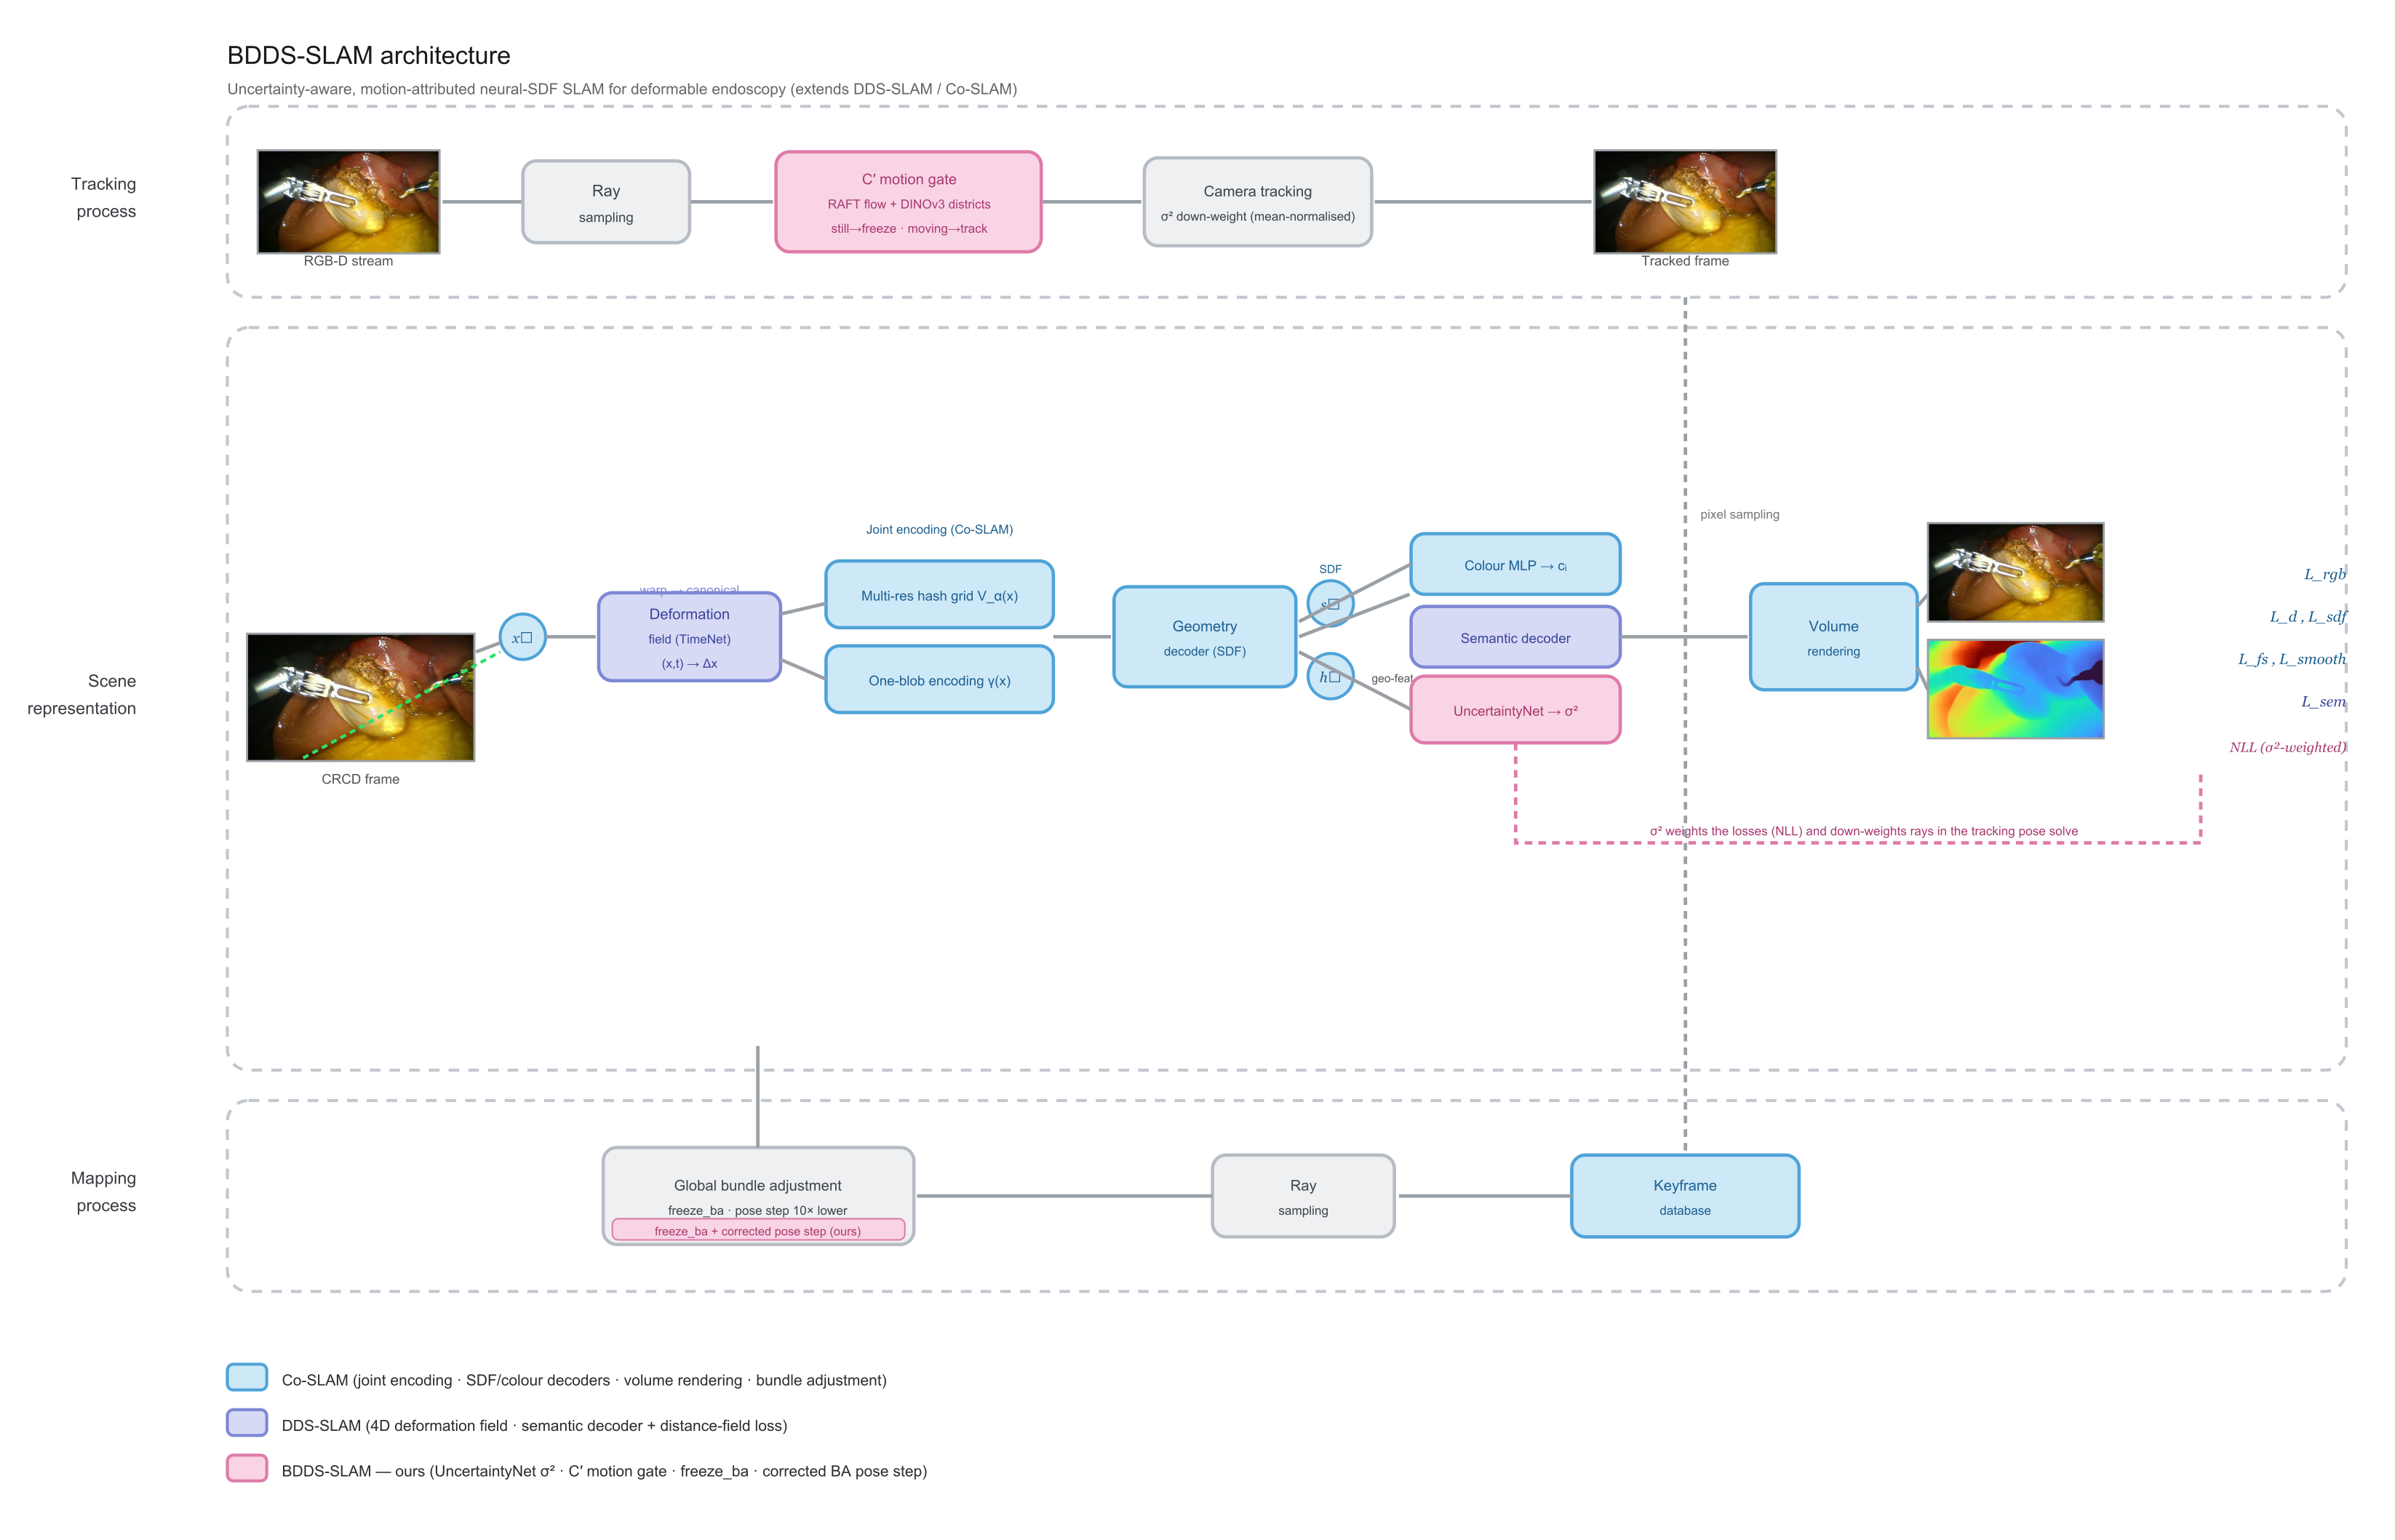
\includegraphics[width=\linewidth]{figures/did_overview.png}
    \caption{Overview of DID-SLAM: the Co-SLAM/DDS-SLAM neural-SDF substrate augmented with two flag-gated contributions --- a learned aleatoric uncertainty (Section~\ref{sec:uncertainty}) and a label-free motion attribution whose freeze is re-pinned after every bundle-adjustment cycle (Section~\ref{sec:motion}) --- together with a corrected bundle-adjustment configuration (Section~\ref{sec:hyperparams}).}
    \label{fig:did_overview}
\end{figure}
\FloatBarrier
\subsection{Uncertainty-Aware Down-Weighting}
\label{sec:uncertainty}
The first contribution transfers the aleatoric-uncertainty principle --- introduced for distractor-free NeRF reconstruction by NeRF On-the-go~\cite{Ren2024} and carried into Gaussian-splatting SLAM by WildGS-SLAM~\cite{Zheng2024} --- onto a neural-SDF SLAM substrate, using a learned uncertainty to attenuate unreliable measurements in both mapping and tracking. A lightweight head predicts a per-ray variance $\sigma^2(r)$ from the geometry feature $h$; under a Gaussian observation model, the head is trained by the negative log-likelihood (NLL) of the photometric residual~\cite{KendallGal2017}:
\begin{equation}
    \mathcal{L}_{\text{NLL}} = \frac{1}{N}\sum_{r}\frac{1}{2}
    \left(\frac{\|C(r)-\hat{C}(r)\|^2}{\sigma^2(r)} + \log\sigma^2(r)\right)
    \label{eq:nll}
\end{equation}
The $1/\sigma^2$ term rewards small residuals where the model is confident, while the $\log\sigma^2$ term penalises blanket high variance; the head therefore learns to raise $\sigma^2$ where the residual is irreducibly large --- the deforming and independently-moving regions the static field cannot explain.

The learned variance is consumed by both elements of the system. During mapping it enters directly through \eqref{eq:nll}, so high-uncertainty rays contribute proportionally less to the field optimisation. During tracking, where the map is fixed and only the six camera-pose parameters vary, the same variance is converted into a per-ray trust weight that down-weights unreliable rays in the pose solve:
\begin{equation}
    w(r) = \mathrm{clamp}\!\left(\frac{1}{\sigma^2(r)},\; w_{\min},\; w_{\max}\right),
    \label{eq:unc-weight}
\end{equation}
applied multiplicatively to the per-ray colour and depth residuals. The weight is detached from the optimisation graph, so $\sigma^2$ acts purely as an attenuation and does not itself back-propagate into the pose.

Two guards control the weight. First, on rays where the map holds an accumulated rendering opacity below $0.5$, $\sigma^2$ sits at its clamp floor and \eqref{eq:unc-weight} would assign such rays \emph{maximum} trust; since a ray without a surface carries no reliable pose information, its weight is instead reset to the neutral value $w = 1$. Second, the weight vector is mean-normalised, $w \leftarrow w / \bar{w}$, so that the down-weighting \emph{redistributes} trust across the sampled rays at a fixed total rather than silently rescaling the photometric terms against the geometric ones in \eqref{eq:coslam-total}. A single uncertainty estimate thus acts as both a mapping regulariser and a tracking robustifier, reducing the influence of deforming tissue and moving instruments wherever they would otherwise corrupt the estimate.

\begin{figure}[!ht]
    \centering
    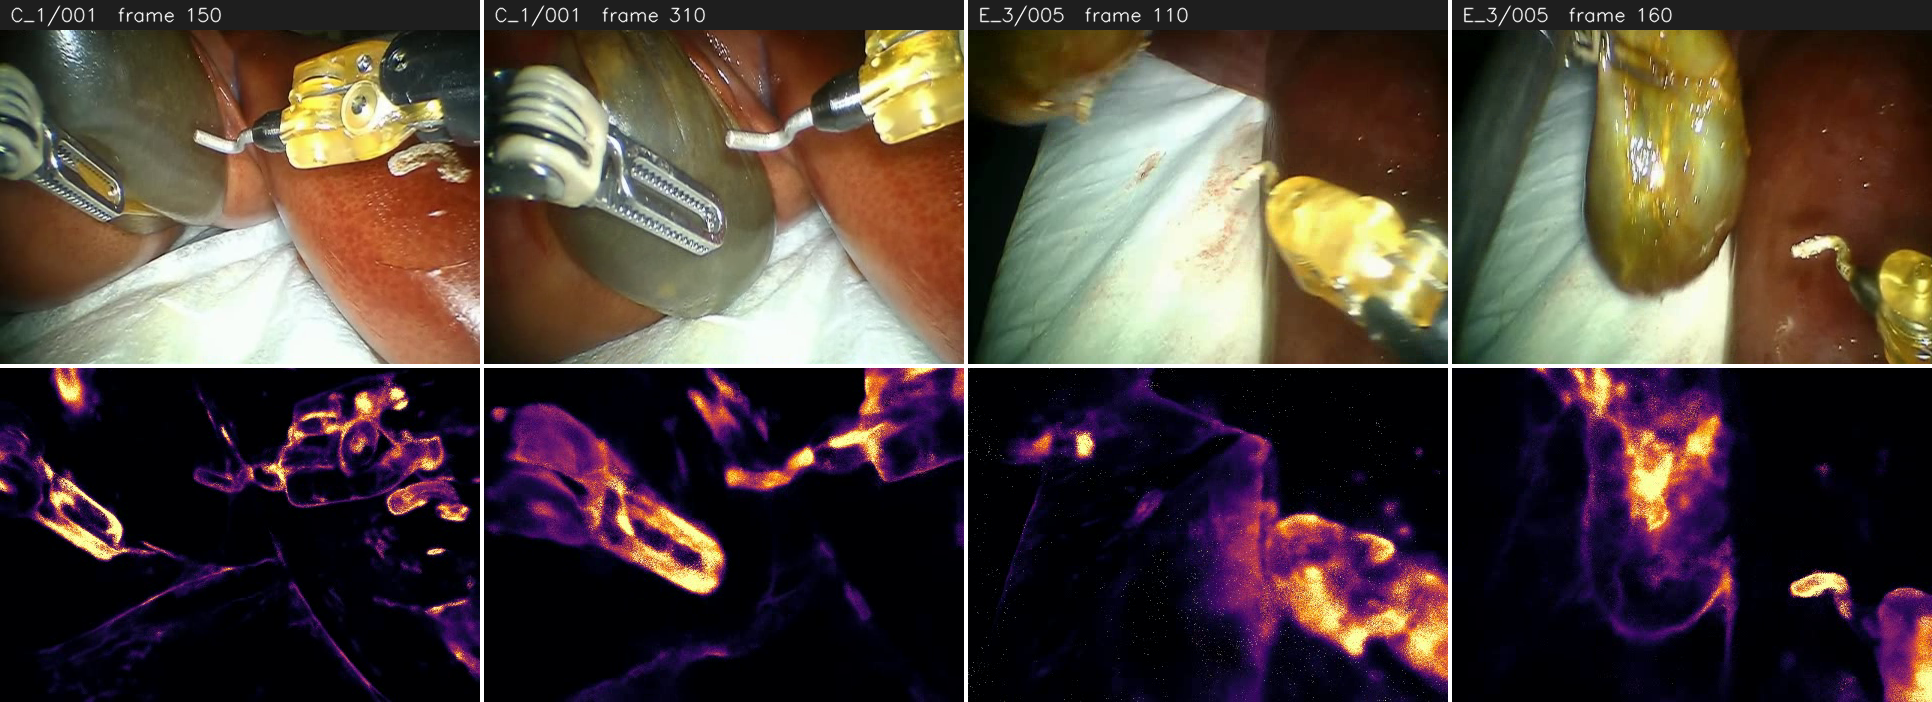
\includegraphics[width=1\linewidth]{figures/uncertainty_downweight.png}
    \caption{Uncertainty-aware down-weighting. A lightweight head predicts a per-ray variance $\sigma^2$ from the geometry feature $h$, trained by the aleatoric NLL \eqref{eq:nll}. The learned variance is applied as a per-ray trust weight $w = 1/\sigma^2$ \eqref{eq:unc-weight} that attenuates unreliable rays in both halves of the system: the mapping loss and the tracking pose solve.}
    \label{fig:uncertainty_downweight}
\end{figure}
\FloatBarrier
\subsection{Motion Attribution}
\label{sec:motion}
The second contribution decides, for every frame, whether the camera is moving and which regions move independently of it, and gates the pose solve accordingly.
\paragraph{Semantic districts.} A frozen self-supervised vision transformer (base DINOv3-B/16~\cite{Simoni2025}; the choice of backbone is examined below) produces a patch feature grid; its $\ell_2$-normalised rows are clustered into $K$ districts with k-means. Districts are \emph{semantic} rather than spatial: an instrument votes as one bloc regardless of where it lies in the frame, which lets independent movers self-identify without a mask.

\begin{figure}[!ht]
    \centering
    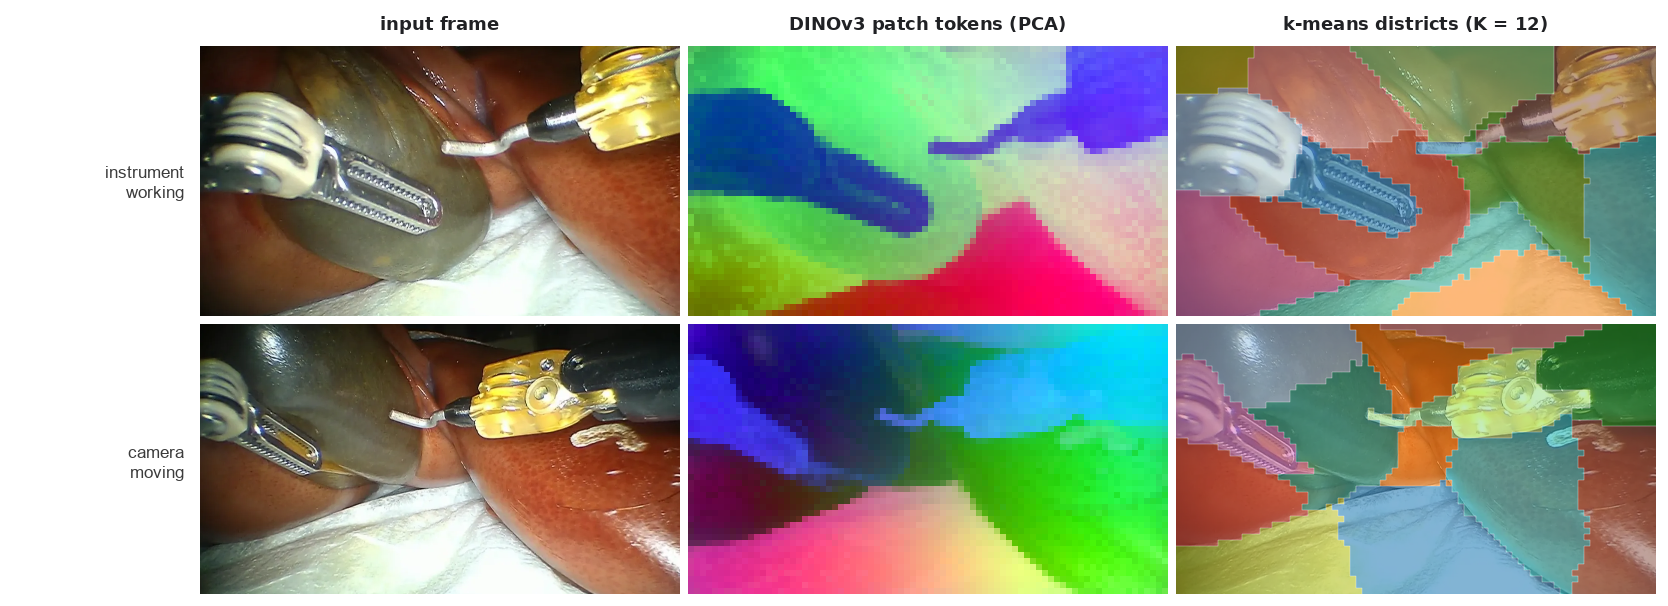
\includegraphics[width=\linewidth]{figures/fig_dino_districts.png}
    \caption{From features to districts. Left: the input frame. Centre: PCA projection of the DINOv3-B/16 patch tokens, the instruments feature-distinct from the tissue they touch. Right: the $K = 12$ k-means districts the deployed gate computes from those tokens (Section~\ref{sec:motion}).}
    \label{fig:dino_districts}
\end{figure}
\FloatBarrier

Optical flow is computed with RAFT~\cite{Teed2020} between the current frame and a reference frame $\delta$ frames earlier ($\delta = 8$), integrating motion well above the flow noise floor on these slow-moving sequences. Each valid district $k$ then casts a vote of its median flow $f_k$, median depth $Z_k$, and centroid $p_k$; the median makes each vote robust to its own outlier pixels. A single tiny egomotion model is fit across the district votes, with regressors chosen so that each motion type carries a distinct depth signature:
\begin{equation}
    f_k \;\approx\; u \;+\; v\,\zeta_k \;+\; d\,r_k\,\zeta_k,
    \qquad \zeta_k = \frac{Z_{\text{med}}}{Z_k},
    \quad r_k = \frac{p_k - p_0}{r_{\text{norm}}}
    \label{eq:vote-fit}
\end{equation}
where $p_0$ is the image principal point and $r_{\text{norm}}$ a normalising radius. Here $u$ is depth-blind, i.e., camera rotation shifts every district equally, $v$ a depth-scaled slide (lateral translation moves near districts more, as $1/Z$), and $d$ a depth-scaled radial zoom (forward motion expands the field). Because $\zeta_k$ is a ratio of depths it is dimensionless, so the unknown global scale of the monocular depth cancels.

\begin{figure}[!ht]
    \centering
    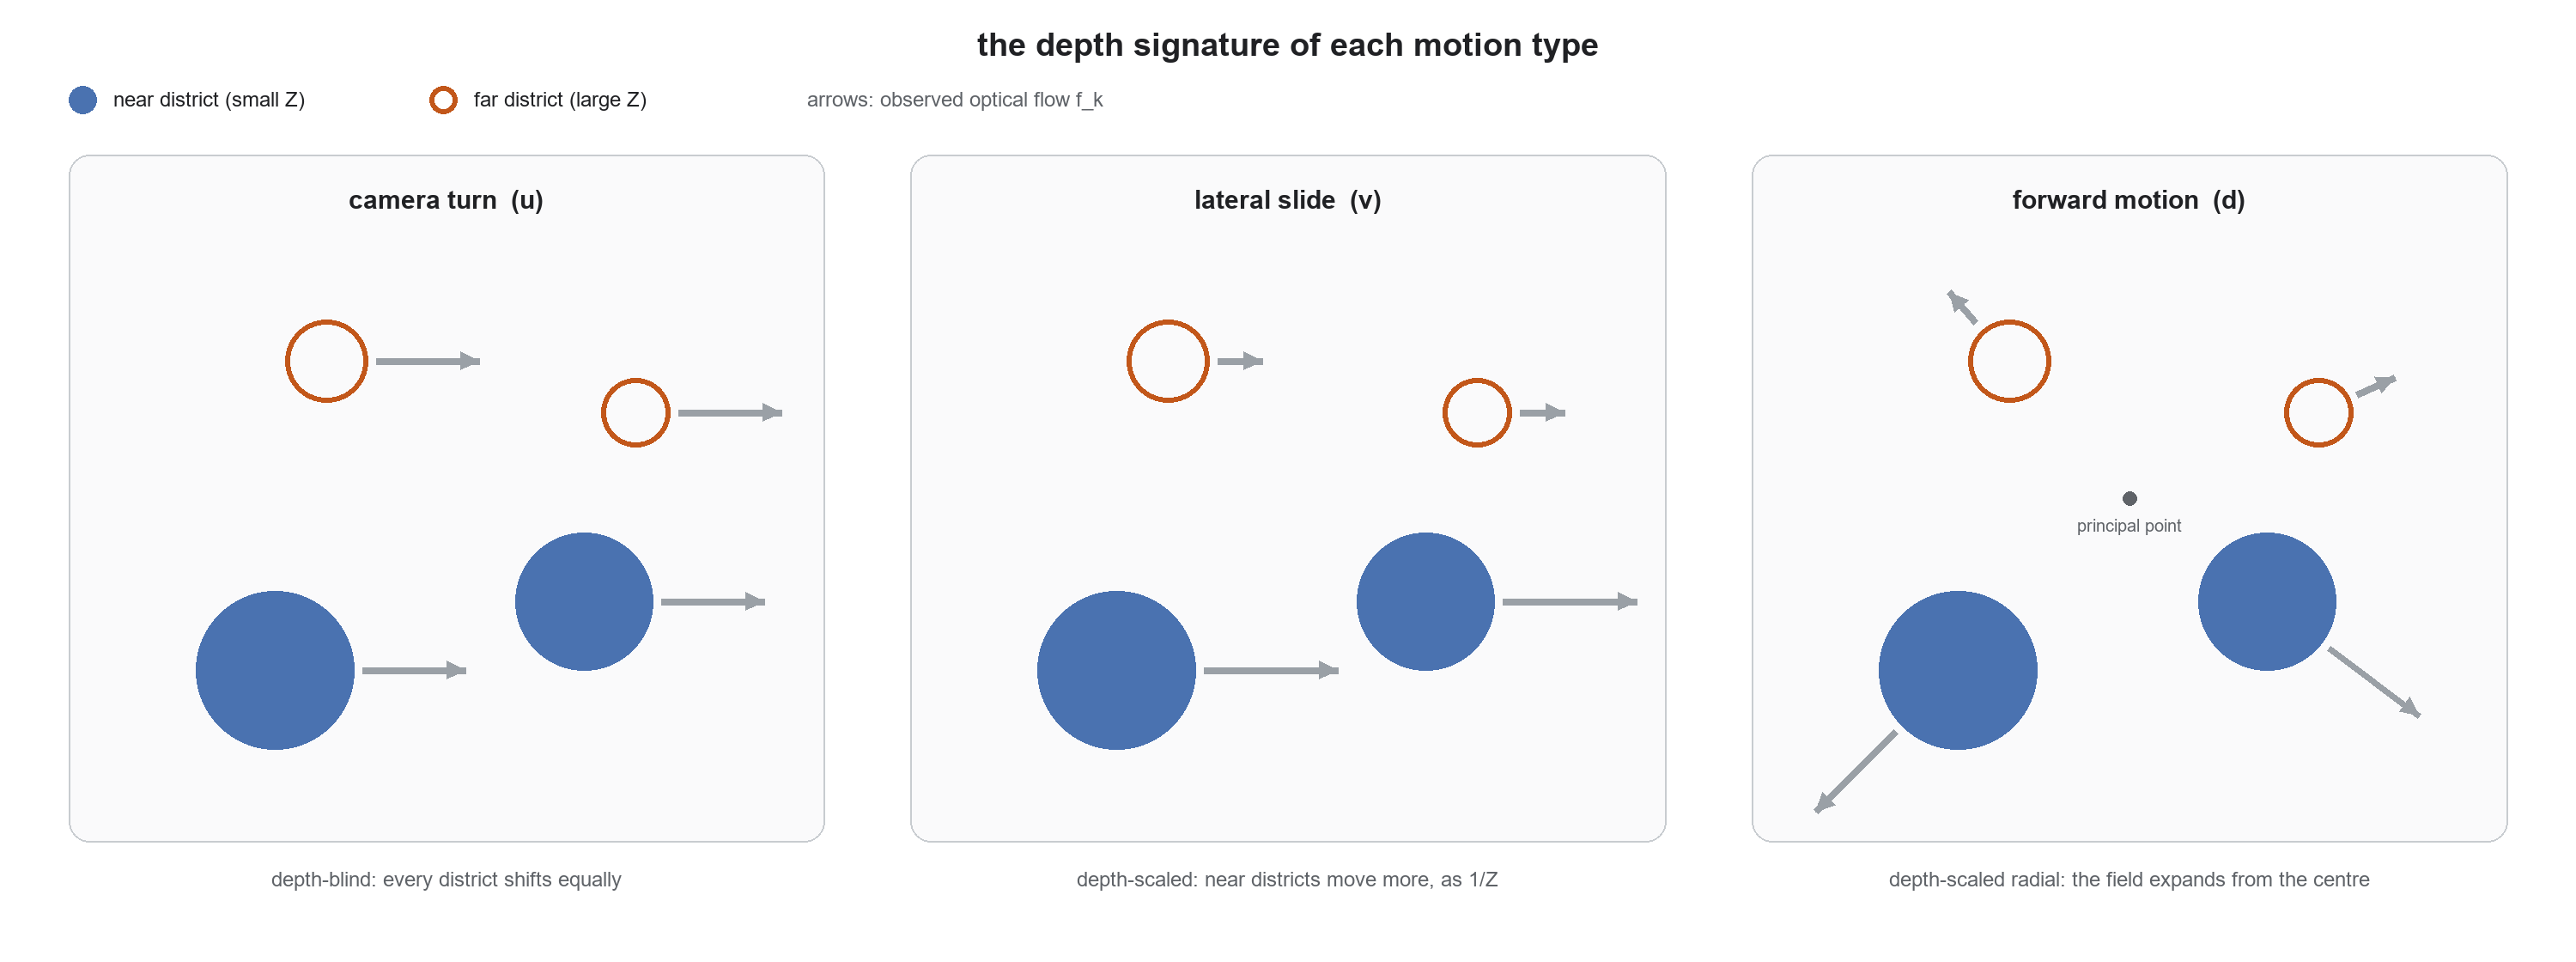
\includegraphics[width=1\linewidth]{figures/depth_signature.png}
    \caption{The three motions the egomotion fit \eqref{eq:vote-fit} separates by their depth signature: rotation (uniform shift), lateral slide ($1/Z$), and forward zoom (radial). Fitting all three cancels the unknown global depth scale.}
    \label{fig:depth_signature}
\end{figure}

The model is fit by least squares and made robust by a median-absolute-deviation reweighting: districts that fit no camera motion (tools and deforming tissue) fall out as outliers and receive a low trust
\begin{equation}
    w_k = \frac{1}{1 + \big(\max(0,\rho_k - \mathrm{med})/\mathrm{scale}\big)^2},
    \qquad \rho_k = \|f_k - \hat{f}_k\|.
    \label{eq:vote-trust}
\end{equation}
Two metrics of the votes decide whether the camera is still: a minority test $q_{10}$, which looks at the tenth-percentile districts' flow magnitudes, and a majority test $\mathrm{dis3}$, the fraction of districts inconsistent in the Sampson (epipolar) sense~\cite{Hartley2004} with a single fundamental matrix $F$ fit to the dense flow:
\begin{equation}
    q_{10} = P_{10}\big(\{\|f_k\|\}\big), \qquad
    \mathrm{dis3} = \frac{|\{k : \mathrm{Sampson}(F,k) > 3\,\text{px}\}|}{|\{\text{valid }k\}|}
    \label{eq:vote-stats}
\end{equation}
\begin{equation}
    \textbf{freeze} \iff q_{10} < \tau_q \;\;\textbf{or}\;\; \mathrm{dis3} > \tau_d
    \qquad (\tau_q = 2.5\,\text{px},\; \tau_d = 0.5)
    \label{eq:cprime}
\end{equation}
The minority test encodes that stillness requires the quietest districts to agree the world is still, so a single large deformation against an otherwise still scene does not imply the camera moved; the majority test asks whether any one rigid-camera story explains the motion. They are combined disjunctively because requiring both simultaneously restores precision on one motion regime only by destroying recall on the other.

When \eqref{eq:cprime} decides that the camera is still, the pose is copied from the previous frame, the solve is skipped, and the frame's relative pose against its anchoring keyframe is refreshed; mapping still runs. Keyframe poses anchor the non-keyframes between them, and the global bundle adjustment re-optimises every keyframe on every cycle, to prevent anchored keyframes from drifting. Gate-frozen keyframes are therefore re-pinned to their frozen pose after every bundle-adjustment cycle, which prevents the pose from jumping: otherwise BA would re-optimise a frozen pose and move it.

\begin{figure}[!ht]
    \centering
    \includegraphics[width=\linewidth]{figures/fig_motion_agreement.png}
    \caption{The gate on three regimes (Section~\ref{sec:motion}): \textbf{C\_1/001} still, votes near zero, pose frozen; \textbf{C\_2/001} moving, votes consistent with one rigid story, tracked; \textbf{E\_3/005} deforming, votes large but the majority epipolar-inconsistent, frozen. Panel statistics use an offline dense-flow proxy; the live values are logged by the gate.}
    \label{fig:motion_agreement}
\end{figure}
\FloatBarrier

The thresholds in \eqref{eq:cprime} are calibrated offline rather than tuned in the loop. We log the per-frame statistics for $(q_{10}, \mathrm{dis3})$ during a run; sweeping these logs against the ground-truth camera motion yields the precision and recall of every candidate operating point $(\tau_q, \tau_d)$, i.e., how successfully we freeze the camera. One discretisation detail matters: with $K = 12$ districts, $\mathrm{dis3}$ is quantised to twelfths, so a strict inequality at $\tau_d = 0.5$ excludes frames on which exactly half the districts disagree (i.e., the majority must agree).

\paragraph{Feature Generation.} The districts are built from a frozen feature generator. This decision rests on two tests. First, a probe-margin test scored each backbone by the mean cosine similarity of a probe patch on the mover to the rest of the moving region, minus its similarity to everything else. DINOv2-S/14 with registers~\cite{Oquab2023,Darcet2024} ranked the highest at $+0.33$, the base DINOv3-B/16~\cite{Simoni2025} $+0.29$, and a DINOv3 backbone fine-tuned for surgical segmentation only $+0.07$ when tested at its final layer. The fine-tuned collapse is expected; a segmentation objective pulls all features of a class together, which removes the intra-tissue variation the clustering relies on. The first result is therefore that the featuriser should not be fine-tuned; a raw backbone creates better features than a fine-tuned one; the features and their cosine similarities are shown in Figure~\ref{fig:dino_comparison}.
\begin{figure}[!ht]
    \centering
    \includegraphics[width=\linewidth]{figures/fig_dino_comparison.png}
    \caption{What each backbone sees. Rows: DINOv2-S/14, base DINOv3-B/16 (the final model's featuriser), and the surgical-segmentation fine-tune of DINOv3 at its final layer. Columns: the input frame (yellow circle: the probe patch on the instrument); the PCA of the patch tokens; the cosine similarity of every patch to the probe; and the PCA on a camera-moving frame. The raw backbones keep the instrument feature-distinct from the tissue; the fine-tune has collapsed (Section~\ref{sec:motion}).}
    \label{fig:dino_comparison}
\end{figure}
However, running both raw backbones end-to-end on the evaluation sequences, the freeze decision is near-identical: $q_{10}$ correlates at $0.99$ between DINOv2-S/14 and base DINOv3-B/16, $\mathrm{dis3}$ is effectively the same, and $94$--$95\%$ of the freeze decisions agree. The $5$--$6\%$ that differ reflect base DINOv3 performing slightly above DINOv2, with higher freeze precision and recall on both design sequences and a small tracking improvement on the deforming sequence.

\paragraph{Per-ray trust variants (ablated: redundant behind the freeze gate).} The same votes support a softer consumer: the fit residuals of \eqref{eq:vote-trust}, or a depth-normalised deviation from the district consensus, can be painted into a dense per-ray motion trust and applied in the pose solve multiplicatively with the uncertainty weight of \eqref{eq:unc-weight} on tracked frames. These variants are evaluated in the ablations and not retained in the locked configuration, for measured reasons. Behavioural audits against kinematic ground truth showed the depth-pooled variant responds to camera rotation rather than to scene motion: its normalisation is exact for camera-translation parallax, which scales as $1/Z$, but mis-scales rotational flow, which is depth-independent. The sharper de-rotated variant discriminates scene motion nearly perfectly on the design sequences, but discrimination is not the binding constraint: stacking any trust behind the freeze gate starves the solve, because the gate has already removed the confidently-still frames, so the trust mutes precisely the frames that still need tracking. The freeze decision, which removes ambiguous frames outright rather than re-weighting within them, is the consumer that survives measurement.

\paragraph{Zero-motion prior (ablated: no gain over the freeze).} The freeze is a hard, per-frame decision, so a softer companion was evaluated for the drift on frames that are tracked rather than frozen. On near-static sequences the pose solve still over-travels on frames the gate does not freeze: frames that are still but sit just below the threshold, or individual pose axes that the narrow endoscopic geometry leaves weakly observable. A zero-motion prior penalises per-frame pose change directly, adding
\begin{equation}
    \mathcal{L}_{\text{zm}} = \lambda_r \lVert \Delta\mathbf{r} \rVert^2 + \lambda_t \lVert \Delta\mathbf{t} \rVert^2
    \label{eq:zeromotion}
\end{equation}
to the tracking loss, where $\Delta\mathbf{r}$ and $\Delta\mathbf{t}$ are the rotation and translation of the current pose relative to the previous committed pose. The penalty is the same in every direction, but its effect is not. The SDF data term has its own per-axis curvature (approximately the squared flow Jacobian), so an observable axis with a steep gradient overrules the prior and keeps the real motion, while a flat, unobservable axis is pinned towards zero. The prior is added before the best-iterate selection so that it binds, and $\lambda_r$ and $\lambda_t$ are calibrated against the SDF loss scale. Evaluated on the design sequences, the prior brought no further gain: the drift it targets is already removed by the freeze and the corrected bundle-adjustment configuration, and it is not retained in the final configuration.

\FloatBarrier
\begin{figure}[!ht]
    \centering
    \includegraphics[width=\linewidth]{figures/fig_vote_pipeline.png}
    \caption{The label-free motion-attribution pipeline (Section~\ref{sec:motion}): a frame pair yields ViT districts, RAFT flow~\cite{Teed2020} and up-to-scale depth; each district's median vote $(f_k, Z_k, p_k)$ feeds the depth-signature fit \eqref{eq:vote-fit}, whose statistics \eqref{eq:vote-stats} drive the freeze decision \eqref{eq:cprime}. Frozen keyframes are re-pinned after each bundle-adjustment cycle.}
    \label{fig:vote_pipeline}
\end{figure}
\FloatBarrier

\subsection{Evaluation Metrics}
\label{sec:eval_metrics}

Evaluation covers both elements of a SLAM system --- \emph{tracking} (camera-pose accuracy) and \emph{mapping} (reconstruction quality, judged through rendering) --- plus behavioural diagnostics and segmentation accuracy. Quantitative results use a single random seed ($n{=}1$); measured baseline seed-to-seed spread is quoted alongside the result, and the single-seed protocol is discussed as a limitation in Section~\ref{sec:discussion}.

\subsubsection{Tracking: Sim(3) Absolute Trajectory Error}
\label{sec:eval_ate}

The primary tracking metric is Absolute Trajectory Error (ATE) after a \emph{similarity} (Sim(3)) alignment. Given estimated and ground-truth camera centres $\{\mathbf{x}_i\}_{i=1}^{N}$ and $\{\mathbf{y}_i\}_{i=1}^{N}$, paired one-to-one by frame index, the Umeyama closed-form solution \cite{umeyama1991} recovers the scale $s$, rotation $R$ and translation $\mathbf{t}$ minimising
\begin{equation}
(s^\ast, R^\ast, \mathbf{t}^\ast) \;=\; \operatorname*{arg\,min}_{s,R,\mathbf{t}} \sum_{i=1}^{N} \bigl\lVert \mathbf{y}_i - \left( sR\,\mathbf{x}_i + \mathbf{t} \right) \bigr\rVert^2 ,
  \label{eq:umeyama}
\end{equation}
via the SVD of the centred cross-covariance $H = \sum_i (\mathbf{x}_i - \bar{\mathbf{x}})(\mathbf{y}_i - \bar{\mathbf{y}})^{\!\top} = U S V^{\!\top}$, with $R^\ast = V \operatorname{diag}(1,1,\det(VU^{\!\top}))\, U^{\!\top}$ and the scale $s^\ast$ given by the ratio of the (sign-corrected) singular-value sum to the estimate's centred variance. The per-frame error and its summary are then
\begin{equation}
e_i = \bigl\lVert \mathbf{y}_i - \left( s^\ast R^\ast \mathbf{x}_i + \mathbf{t}^\ast \right)\bigr\rVert, \qquad \mathrm{ATE}_{\mathrm{RMSE}} = \sqrt{\tfrac{1}{N}\textstyle\sum_i e_i^2},
\end{equation}
reported in millimetres alongside the mean, median and maximum.

\subsubsection{Tracking: scale-free shape diagnostics}
\label{sec:eval_shape}

CRCD ground-truth camera motion is small (path lengths ${\sim}20$--$80$\,mm, i.e.\ ${\sim}0.05$--$0.4$\,mm/frame), near or below the tracker's noise floor (\emph{sub-SNR}). Here a small ATE can be achieved by a trajectory that is merely \emph{compact} rather than \emph{correct}, so ATE alone is insufficient; two complementary, scale-free diagnostics are always reported with it:

\paragraph{Path-length ratio.} With $L(\mathbf{z}) = \sum_i \lVert \mathbf{z}_{i+1} - \mathbf{z}_i \rVert$ the trajectory arc length,
\begin{equation}
\rho_{\mathrm{path}} \;=\; \frac{s^\ast \, L(\mathbf{x})}{L(\mathbf{y})}
\end{equation}
measures over- or under-travel after scale correction. $\rho_{\mathrm{path}} > 1$ indicates excess accumulated motion (jitter or exaggerated steps); $\rho_{\mathrm{path}} \to 0$ exposes a degenerate ``frozen'' trajectory that ATE alone would reward on near-static sequences.

\paragraph{Aligned per-axis correlation.} The absolute Pearson correlation $|r|$ between the \emph{Sim(3)-aligned} estimate and the ground truth along the dominant motion axis, together with the mean over all three axes. Correlation is invariant to rescaling, so this isolates \emph{shape} tracking from any residual scale artefact. Alignment is essential: because Sim(3) alignment includes a rotation, correlating the \emph{raw} estimate against the ground truth compares physically different axes and can read near zero even when the aligned trajectory tracks well; this artefact was observed and corrected in this work.

\subsubsection{Rendering: PSNR, SSIM, LPIPS}
\label{sec:eval_render}

Mapping quality is judged by re-rendering every training view from the final model against the input frames, using the standard triplet.

\paragraph{PSNR} (peak signal-to-noise ratio), on images in $[0,1]$:
\begin{equation}
\mathrm{PSNR} = 20 \log_{10}\!\left( \frac{1}{\sqrt{\mathrm{MSE}}} \right), \qquad \mathrm{MSE} = \tfrac{1}{|\Omega|}\textstyle\sum_{p \in \Omega} \bigl( I(p) - \hat{I}(p) \bigr)^2 ,
\end{equation}
a purely pixel-wise fidelity measure (higher is better).

\paragraph{SSIM} (structural similarity \cite{Wang2004}) compares local luminance, contrast and structure statistics computed under an $11{\times}11$ Gaussian window ($\sigma{=}1.5$):
\begin{equation}
\mathrm{SSIM}(p) = \frac{(2\mu_1\mu_2 + C_1)(2\sigma_{12} + C_2)} {(\mu_1^2 + \mu_2^2 + C_1)(\sigma_1^2 + \sigma_2^2 + C_2)},
\end{equation}
with $C_1 = 0.01^2$, $C_2 = 0.03^2$, averaged over the image (higher is better). SSIM is less sensitive than PSNR to uniform brightness shifts and more sensitive to structural degradation (blur, ghosting).

\paragraph{LPIPS} (learned perceptual image patch similarity \cite{zhang2018lpips}) embeds both images with a fixed pre-trained CNN and measures the weighted $\ell_2$ distance between normalised deep features across layers $l$:
\begin{equation}
\mathrm{LPIPS}(I, \hat{I}) = \sum_l \frac{1}{H_l W_l} \sum_{h,w} \bigl\lVert w_l \odot \bigl( \phi_l(I)_{hw} - \phi_l(\hat{I})_{hw} \bigr) \bigr\rVert_2^2
\end{equation}
(lower is better). LPIPS correlates with human judgement where PSNR/SSIM fail: a render can be blurry-but-average (good PSNR, poor LPIPS) or sharp with small misalignments (poor PSNR, good LPIPS); reporting all three disambiguates which regime a change lives in.

On Semantic-SuPer sequences the supplied ``ground-truth'' poses are placeholder identities, so tracking metrics are meaningless and rendering metrics are the sole arbiter; CRCD provides kinematic camera poses, so both halves are evaluated.

\subsubsection{Depth-$L_1$ (self-consistency)}
\label{sec:eval_depth}

CRCD ships no measured ground-truth depth: the depth input is itself generated (MoGe-2). Depth-$L_1$ is therefore defined \emph{input-versus-output, per model}: the mean absolute difference (in mm) between the depth a model \emph{renders} and the depth it was \emph{given} on that frame,
\begin{equation}
\mathrm{Depth}\text{-}L_1 = \tfrac{1}{|\mathcal{V}|} \sum_{p \in \mathcal{V}} \bigl| \hat{D}(p) - c\,D_{\mathrm{in}}(p) \bigr| ,
\end{equation}
where $\mathcal{V}$ masks invalid pixels ($\leq 0$ or outside a plausible metric range in either map) and $c$ is the model's own depth pre-scaling factor, so both maps live in the model's own frame. This is explicitly a \emph{self-consistency} measure (how faithfully the reconstruction absorbed its geometric supervision), not an accuracy-versus-reality measure, and is stated as such wherever quoted.

\subsubsection{Segmentation: mean Intersection-over-Union}
\label{sec:eval_miou}

Semantic components (the DINO-based segmentation heads of the benchmarked semantic-SLAM baselines) are evaluated by class-wise Intersection-over-Union over the four CRCD classes $\{$background, liver, gallbladder, tool$\}$,
\begin{equation}
\mathrm{IoU}_c = \frac{|P_c \cap G_c|}{|P_c \cup G_c|}, \qquad \mathrm{mIoU} = \tfrac{1}{4} \textstyle\sum_c \mathrm{IoU}_c ,
\end{equation}
accumulated over all pixels of the evaluation set. Generalisation is judged under a leave-one-snippet-out protocol: each benchmark snippet's head is trained on the remaining snippets (with two held out as an inner validation set for model selection, avoiding the leakage of a random frame-level split) and tested on the never-seen snippet. For the four single-snippet episodes this equals leave-one-\emph{episode}-out and yields a true cross-patient number; the one snippet sharing an episode with training data is in-domain and reported separately from the cross-episode headline mean.

\section{Experiments and Results}
\subsection{Experimental Setup}
\label{sec:setup}

\subsubsection{Evaluation sequences}

All experiments use the CRCD sequence dataset of Section~\ref{sec:data_packs}. From the twenty published snippets we select five, drawn from five episodes to span the distinct problems a surgical SLAM system must handle (Table~\ref{tab:eval_sequences}; motion statistics follow Table~\ref{tab:motion}).

\begin{table}[!ht]
\centering
\caption{Evaluation sequences and their roles. Frames and motion statistics are taken from Table~\ref{tab:motion}; ``still'' is the fraction of frames below the motion-frame velocity thresholds of Section~\ref{sec:motion_analysis}.}
\label{tab:eval_sequences}

\resizebox{\textwidth}{!}{%
\begin{tabular}{l r r r l}
\toprule
\textbf{Sequence} & \textbf{Frames} & \textbf{Still} & \textbf{Path (mm)} & \textbf{Description} \\
\midrule
C\_1/001 & 360  & 60\% & 18.6 & short, easy to track; large deformations \\
C\_2/001 & 730  & 54\% & 56.3 & largest camera travel \\
C\_3/001 & 1527 & 74\% & 78.8 & long, predominantly still \\
E\_3/005 & 265  & 49\% & 43.5 & large and fast tissue/tool motion \\
G\_3/001 & 1987 & 82\% & 31.6 & close-up footage --- long sequence \\
\bottomrule
\end{tabular}%
}

\end{table}



\subsubsection{Data preparation}

Sequences pass through a staging pipeline run once per sequence and cached. Frames are rectified with the published ECM stereo calibration (Section~\ref{sec:data_packs}); per-frame depth is generated with MoGe-2 on the rectified left frames and anchored to metric scale by stereo matching on the rectified pairs at 120-frame intervals, with a consistency gate rejecting sequences whose anchors disagree (where the scaling changes significantly between intervals); scene bounds follow from the resulting metric depth; and the published semantic rasters are rectified alongside the imagery, giving the four-class map (background, liver, gallbladder, instrument) consumed by the semantic and instrument-masking components.

\subsubsection{Implementation}

All experiments run a single code base forked from the public DDS-SLAM release~\cite{Shan2024}, with every modification gated behind a configuration flag defaulting to \emph{off}. A bit-identical regression gate (identical random-number state after model construction, identical parameter counts, identical \texttt{state\_dict} keys against the upstream commit) guarantees the unmodified configuration reproduces the released implementation exactly, so the baseline is a provably untouched control and every measured difference is attributable to exactly one enabled component. Experiments run on Google Colab GPUs (Tesla T4, 15\,GB; A100, 40\,GB and 80\,GB for the largest configurations) under PyTorch~2.x / CUDA~12.x, with the tiny-cuda-nn hash-encoding backend rebuilt for the resident GPU architecture. TF32 tensor-core arithmetic is disabled throughout: the SDF and pose optimisation are precision-sensitive, and TF32 introduced run-to-run nondeterminism on A100-class hardware. Every run emits a fixed artefact set (rendered frames, the estimated trajectory, per-frame diagnostics, a composite diagnostic video), and all evaluation uses a common tool chain (Section~\ref{sec:eval_metrics}) applied identically to every arm.

\subsubsection{Hyperparameters}
\label{sec:hyperparams}

The final configuration is one hyperparameter set shared by all five sequences; per-sequence tuning is avoided, since the freeze mechanism must generalise to motion regimes it has not seen. Table~\ref{tab:hyperparams} lists the major choices with the reasoning behind each: the learning rates and initialisation governing the pose solve, and the parameters introduced by the two contributions. Adapting the released DDS-SLAM configuration to the CRCD required further departures from its defaults beyond those tabulated: decoder capacity, mapping-iteration schedule and SDF voxel size, chosen once for the resolution and scene scale of this dataset. These are held identical across the base and DID-SLAM arms, forming part of the common substrate rather than a difference under test, so every measured difference in Section~\ref{sec:results_main} remains attributable to the flag-gated components alone. Every value was locked on the two design sequences before the held-out runs.

\begin{table}[!ht]
\centering
\caption{Hyperparameters of the final configuration that depart from the released DDS-SLAM defaults, with the reasoning for each choice. All values were locked on the design sequences (C\_1/001, E\_3/005) before any held-out sequence was run.}
\label{tab:hyperparams}
\small
\resizebox{\textwidth}{!}{%
\begin{tabular}{l l l p{6.2cm}}
\toprule
Parameter & DDS-SLAM & DID-SLAM & Reasoning \\
\midrule
BA pose learning rate & $10^{-4}$ & $10^{-5}$ & reduces the pose noise floor introduced by the Adam optimiser \\
Constant-velocity initialisation & on & off & inter-frame motion ($0.16$--$0.33$\,mm) sits far inside the tracker's per-frame reach; the extrapolation carries optimiser artefact rather than motion signal \\
Gate thresholds $(\tau_q, \tau_d)$ & --- & $(2.5\,\text{px},\, 0.5)$ & offline precision/recall sweep of the logged per-frame statistics against ground-truth camera motion (Section~\ref{sec:motion}); $\tau_d$ placed between attainable twelfths of the quantised statistic \\
Districts $K$ / reference stride $\delta$ & --- & $12$ / $8$ & $\delta = 8$ integrates flow well above its noise floor on these slow sequences; $K = 12$ keeps districts large enough for stable median votes \\
Uncertainty clamp $[w_{\min}, w_{\max}]$ & --- & $[0.1,\, 10]$ & bounds keep the down-weight a redistribution of trust rather than a hard mask (Section~\ref{sec:uncertainty}) \\
NLL weight & --- & $0.1$ & keeps the $\sigma^2$ head a regulariser, subordinate to the photometric loss \\
Hash table size & $2^{16}$ & $2^{19}$ & removes hash collisions visible as render blur at $1280 \times 720$ \\
Photometric loss & L2 & Charbonnier & robust to the specular outliers endemic to endoscopy \\
\bottomrule
\end{tabular}}
\end{table}
\FloatBarrier

\subsection{Evaluation of Tracking and Reconstruction}
\label{sec:results_main}

The final DID-SLAM configuration was locked on the two design sequences (C\_1/001 and E\_3/005). The remaining three (C\_2/001, C\_3/001, G\_3/001) were then run once, unseen, as a held-out generalisation test against the unmodified DDS-SLAM base under the identical staging and evaluation pipeline; the freezing mechanism requires a single hyperparameter set rather than one tuned per sequence, so that the model performs suitably on unseen data. Table~\ref{tab:results_main} reports the full battery.

\begin{table}[!ht]
\centering
\caption{DID-SLAM (final configuration) against the unmodified DDS-SLAM base on the five evaluation sequences, single seed, with base and DID-SLAM scored under the identical Sim(3) evaluation. The base row is the benchmark-staged DDS-SLAM run of Table~\ref{tab:results_sota}. Sim(3) ATE$_{\mathrm{RMSE}}$ in mm; path ratio, aligned $|r|_{\mathrm{dom}}$ and rendering metrics per Section~\ref{sec:eval_metrics}. The three held-out sequences were never used during development.}
\label{tab:results_main}
\resizebox{\textwidth}{!}{%
\begin{tabular}{l l r rrr rr rrrr}
\toprule
& & & \multicolumn{3}{c}{Tracking (ATE, mm)} & & & \multicolumn{4}{c}{DID-SLAM rendering} \\
\cmidrule{4-6} \cmidrule{9-12}
Sequence & Role & $N$ & base & DID & $\Delta$ & path ratio & $|r|_{\mathrm{dom}}$ &
PSNR$\uparrow$ & SSIM$\uparrow$ & LPIPS$\downarrow$ & D-$L_1$ \\
\midrule
C\_1/001 & design   &  360 & 2.64 & \textbf{1.60} & $-39\%$ & 2.23 & 0.985 & 25.49 & 0.813 & 0.437 & 10.14 \\
E\_3/005 & design   &  265 & 5.31 & \textbf{4.69} & $-12\%$ & 3.52 & 0.463 & 24.20 & 0.812 & 0.455 & 15.65 \\
C\_2/001 & held-out &  730 & 6.78 & \textbf{3.93} & $-42\%$ & 1.88 & 0.951 & 21.84 & 0.762 & 0.481 & 11.68 \\
C\_3/001 & held-out & 1527 & 10.25 & \textbf{7.61} & $-26\%$ & 3.05 & 0.820 & 24.39 & 0.828 & 0.424 & 10.67 \\
G\_3/001 & held-out & 1987 & 4.12 & \textbf{2.28} & $-45\%$ & 5.93 & 0.976 & 28.78 & 0.909 & 0.300 & 15.03 \\
\midrule
mean (5) & & --- & 5.82 & \textbf{4.02} & $-31\%$ & 3.32 & 0.839 & 24.94 & 0.825 & 0.419 & 12.63 \\
\bottomrule
\end{tabular}}
\end{table}
\FloatBarrier
DID-SLAM improves tracking on all five sequences, with the largest gains on sequences it never saw during development ($-45\%$ on G\_3/001 and $-42\%$ on C\_2/001, alongside $-26\%$ on C\_3/001; the longest, G\_3/001 at 1987 frames, gives the best of the held-out three at $2.28$\,mm). This was expected: the held-out set is $54$--$82\%$ camera-still, the regime the freeze, its bundle-adjustment re-pin and the corrected pose step were built to handle. Trajectory shape improves alongside error: the aligned dominant-axis correlation on the held-out sequences reaches $0.95$--$0.98$ (C\_2, G\_3) against $0.88$--$0.89$ for the base, and the path ratio on C\_2/001 falls from $8.7$ to $1.9$. As Figure~\ref{fig:did_traj_c2} shows, the base estimate oscillates around the true path while the DID-SLAM estimate follows it.

The reconstruction cost of these gains is small and attributable. DID-SLAM improves SSIM on every sequence (mean $0.825$ against $0.807$) and LPIPS on every sequence (mean $0.42$ against $0.46$), while trailing the base by $0.6$\,dB of PSNR (mean $24.94$ against $25.56$). That PSNR difference is the Charbonnier photometric loss behaving as intended: where the base's L2 objective squares and so chases the specular glints endemic to endoscopy, the robust loss declines to, which costs peak pixel fidelity and buys structural agreement (Section~\ref{sec:hyperparams}). The map meanwhile trains on frozen frames, consistent with the design choice. The base scores better on Depth-$L_1$ on four of the five sequences, and where it does the gap tracks its over-travel: an unconstrained pose adds degrees of freedom that absorb the frame-to-frame inconsistency of the monocular depth, improving input-versus-output self-consistency while corrupting the trajectory; on G\_3/001, where the base over-travels most ($18.3\times$ vs $5.9\times$), the Depth-$L_1$ gap is widest, while on E\_3/005, where the path ratios are comparable, the two are equal. C\_3/001 is the exception that bounds the mechanism: there DID-SLAM wins on Depth-$L_1$ despite the base over-travelling more than twice as far. The deforming sequence remains the hardest: E\_3/005 improves by $12\%$ but keeps the weakest shape correlation ($0.46$), and is the only sequence on which the base's seed-to-seed spread was measured ($\pm 0.60$\,mm); its residual error and the limit it sets on the gate are examined in Section~\ref{sec:discussion}.


\subsection{Ablations}
\label{sec:results_ablations}

Every component of the final configuration was adopted or rejected on the design sequences; Table~\ref{tab:results_abl} summarises the ladder, one change at a time.

\begin{table}[!ht]
\centering
\caption{Component ladder on the design sequences, full battery (Sim(3) ATE$_{\mathrm{RMSE}}$ in mm; path ratio, aligned $|r|_{\mathrm{dom}}$, rendering and Depth-$L_1$ per Section~\ref{sec:eval_metrics}). Single seed throughout except the base on E\_3/005, which is the mean of three seeds. Each row adds one component to the row above; the final model additionally carries the corrected bundle-adjustment configuration (Section~\ref{sec:hyperparams}) and the DINOv3 districts (Section~\ref{sec:motion}). The ladder is a controlled same-pipeline experiment, so its flag-off base row differs slightly from the benchmark-staged base of Tables~\ref{tab:results_main} and~\ref{tab:results_sota}; the within-ladder deltas are what attribute each component.}
\label{tab:results_abl}
\small
\resizebox{\textwidth}{!}{%
\begin{tabular}{l rrr rrrr}
\toprule
Configuration & ATE (mm) & path ratio & $|r|_{\mathrm{dom}}$ & PSNR$\uparrow$ & SSIM$\uparrow$ & LPIPS$\downarrow$ & D-$L_1$ \\
\midrule
\multicolumn{8}{l}{\textbf{C\_1/001}} \\
\midrule
Base model & 2.03 & 5.50 & 0.984 & 25.58 & 0.817 & 0.434 & 9.50 \\
+ uncertainty (Section~\ref{sec:uncertainty}) & 2.10 & 6.76 & 0.978 & 25.61 & 0.814 & 0.430 & 10.13 \\
+ motion attribution (Section~\ref{sec:motion}) & 1.95 & 4.00 & 0.970 & 25.60 & 0.815 & 0.430 & 10.18 \\
Final model & \textbf{1.60} & \textbf{2.23} & 0.985 & 25.49 & 0.813 & 0.437 & 10.14 \\
\midrule
\multicolumn{8}{l}{\textbf{E\_3/005}} \\
\midrule
Base model & 5.49 & 1.95 & 0.401 & 24.43 & 0.814 & 0.456 & 15.63 \\
+ uncertainty (Section~\ref{sec:uncertainty}) & 5.93 & 2.36 & 0.052 & 24.00 & 0.799 & 0.484 & 15.67 \\
+ motion attribution (Section~\ref{sec:motion}) & \textbf{3.66} & 3.17 & 0.756 & 24.02 & 0.806 & 0.464 & 14.33 \\
Final model & 4.69 & 3.52 & 0.463 & 24.20 & 0.812 & 0.455 & 15.65 \\
\bottomrule
\end{tabular}}
\end{table}

The ladder's gains are separable and attributable: the uncertainty head is neutral alone (its E\_3/005 sits within the base's $\pm 0.60$\,mm seed spread) but enables the weighted solve; the motion attribution pays on the deforming sequence ($-33\%$ on E\_3/005); and the corrected bundle-adjustment configuration pays on the still one (the $-18\%$ step from the motion-attribution row to the final on C\_1/001), the combination transferring to the held-out set (Table~\ref{tab:results_main}). The render battery stays essentially flat down the ladder (PSNR within $0.45$\,dB, SSIM within $0.015$ per sequence, the widest step being the uncertainty head on E\_3/005), so every tracking gain comes effectively free of reconstruction cost; the final model returns a little of the motion-attribution row's E\_3/005 gain ($3.66 \to 4.69$\,mm) in exchange for the still-regime correction, the joint trade that wins across the five sequences. The variants evaluated and not retained (the soft per-ray trust consumers, a lowered dissent threshold, $\sigma^2$-weighted bundle adjustment, the zero-motion prior) each failed for a measured, mechanistic reason rather than by tuning accident (Sections~\ref{sec:uncertainty} and \ref{sec:motion}); notably, a lowered dissent threshold produced the single best C\_1/001 of any configuration and was still rejected, because the same setting was the worst on E\_3/005; the final configuration is the one that wins jointly.

\section{Benchmarking against SoTA Semantic-SLAM pipelines}
\label{sec:benchmarking}
DID-SLAM is measured against five SoTA systems spanning the current semantic-SLAM benchmark: Semantic-SuPer, SNI-SLAM, SGS-SLAM, SemGauss-SLAM and PERSEUS. All run on the same five rectified CRCD snippets from the code provided by their authors, with changes limited to input paths, camera intrinsics, and class taxonomy, so no method was re-tuned beyond what running on the CRCD required. Each consumes the same rectified RGB-D stream; metrics follow Section~\ref{sec:eval_metrics}, and per-snippet results are collected in Table~\ref{tab:results_sota}.

\textbf{DDS-SLAM}~\cite{Shan2024} is the model this thesis extends (Section~\ref{sec:ddsslam}): a neural-SDF SLAM with a time-conditioned deformation warp, and the strongest published starting point for deformable endoscopic SLAM. Run unmodified under identical staging, it is the like-for-like reference row in every sub-table.

\textbf{Semantic-SuPer}~\cite{Lin2023} is the deformable-reconstruction representative: a semantic surfel map deformed by an embedded-deformation graph, fitted per frame against depth, photometric and semantic terms. It attacks the same scenes from the opposite direction, deformation-first with the camera assumed static, which is why its trajectory is a camera-motion proxy read from its deformation graph ($\dagger$).

\textbf{SNI-SLAM}~\cite{Zhu2024} is the semantic neural-implicit representative, from the same laboratory as DDS-SLAM: appearance, geometry and semantics fused by cross-attention over multi-resolution feature grids. As the closest architectural match, it isolates what the deformation warp and motion handling add over a static semantic neural field. Its tracking is mid-field with the same over-travel signature as the other render-loss trackers (path ratios $3.0$--$17.8\times$), and its rendering is the weakest of the neural systems here ($12.5$--$15.6$ PSNR): its depth-pinned sampling forms no surface where the tri-plane field is weak, an architectural mismatch with noisy monocular depth rather than an onboarding artefact.

\textbf{SGS-SLAM}~\cite{sgsslam} is the semantic 3D-Gaussian-splatting representative: an explicit Gaussian map with per-Gaussian semantic channels, tracked by rasterisation, placing explicit splatting against the neural-SDF substrate on identical data.

\textbf{SemGauss-SLAM}~\cite{Zhu2025} extends the same splatting lineage with a per-Gaussian semantic feature field distilled from a DINOv2 head, from the same laboratory as DDS-SLAM and SNI-SLAM, and is the most recent semantic-splatting system. Its G\_3/001 run exhausted an A100-80GB at eleven million Gaussians and is reported as did-not-finish.

\textbf{PERSEUS} is a DROID-SLAM~\cite{Teed2022} fork adapted to endoscopy, estimating the camera from dense optical-flow bundle adjustment; it is the SoTA tracking reference for endoscopic SLAM.
\subsection{Comparison with the SoTA benchmark}
\label{sec:results_sota}

Table~\ref{tab:results_sota} places DID-SLAM against the benchmarked systems of Section~\ref{sec:benchmarking}, split per snippet. The methods have two caveats through the table: Semantic-SuPer's trajectory is a camera-motion proxy read out of its deformation graph ($\dagger$), and SGS-SLAM renders only its keyframe set ($*$). Every trajectory, native or proxy, is scored by the identical Sim(3) evaluation, so every ATE in the table is the same statistic.

\begin{table}[!ht]
\centering
\caption{DID-SLAM against the benchmarked systems, one sub-table per snippet. Tracking is Sim(3) ATE$_{\mathrm{RMSE}}$ in mm ($\dagger$: camera-motion proxy, not a native pose); path ratio and aligned $|r|_{\mathrm{dom}}$ per Section~\ref{sec:eval_metrics}. SGS-SLAM renders keyframes only ($*$); its trajectory is native (SplaTAM camera state). Depth-$L_1$ is per-model self-consistency (Section~\ref{sec:eval_depth}) and is not comparable across methods. Dashes: not exported by the method.}
\label{tab:results_sota}
\small
\resizebox{\textwidth}{!}{%
\begin{tabular}{l rrr rrrr}
\toprule
Method & ATE (mm) & path ratio & $|r|_{\mathrm{dom}}$ & PSNR$\uparrow$ & SSIM$\uparrow$ & LPIPS$\downarrow$ & D-$L_1$ \\
\midrule
\multicolumn{8}{l}{\textbf{C\_1/001}} \\
\midrule
\textbf{DID-SLAM (ours)} & \textbf{1.60} & 2.23 & 0.985 & 25.49 & \textbf{0.813} & 0.437 & 10.14 \\
DDS-SLAM (base)~\cite{Shan2024} & 2.64 & 8.11 & 0.951 & \textbf{25.91} & 0.804 & 0.448 & 7.78 \\
PERSEUS & 2.20 & 3.31 & 0.975 & --- & --- & --- & --- \\
SemGauss-SLAM~\cite{Zhu2025} & 6.50 & 3.25 & 0.76 & 20.57 & 0.771 & 0.344 & 22.5 \\
SGS-SLAM$^{*}$~\cite{sgsslam} & 4.18 & 3.39 & 0.939 & 22.45 & 0.803 & \textbf{0.315} & 23.5 \\
SNI-SLAM~\cite{Zhu2024} & 3.33 & 12.65 & 0.945 & 13.27 & 0.564 & 0.792 & 15.1 \\
Semantic-SuPer$^{\dagger}$~\cite{Lin2023} & 3.06 & 18.86 & 0.950 & 12.17 & 0.399 & 0.709 & 3.54 \\
\midrule
\multicolumn{8}{l}{\textbf{C\_2/001}} \\
\midrule
\textbf{DID-SLAM (ours)} & \textbf{3.93} & 1.88 & 0.951 & 21.84 & \textbf{0.762} & \textbf{0.481} & 11.68 \\
DDS-SLAM (base)~\cite{Shan2024} & 6.78 & 8.66 & 0.879 & \textbf{22.57} & 0.728 & 0.552 & 8.72 \\
PERSEUS & 4.07 & 2.93 & 0.976 & --- & --- & --- & --- \\
SemGauss-SLAM~\cite{Zhu2025} & 8.64 & 13.14 & 0.80 & 16.31 & 0.674 & 0.533 & 44.2 \\
SGS-SLAM$^{*}$~\cite{sgsslam} & 7.64 & 8.15 & 0.864 & 17.52 & 0.701 & 0.504 & 41.6 \\
SNI-SLAM~\cite{Zhu2024} & 7.24 & 8.93 & 0.963 & 14.84 & 0.588 & 0.739 & 26.7 \\
Semantic-SuPer$^{\dagger}$~\cite{Lin2023} & 8.32 & 13.93 & 0.890 & 8.72 & 0.162 & 0.882 & 7.2 \\
\midrule
\multicolumn{8}{l}{\textbf{C\_3/001}} \\
\midrule
\textbf{DID-SLAM (ours)} & \textbf{7.61} & 3.05 & 0.820 & 24.39 & \textbf{0.828} & \textbf{0.424} & 10.67 \\
DDS-SLAM (base)~\cite{Shan2024} & 10.25 & 7.08 & 0.833 & \textbf{24.70} & 0.800 & 0.495 & 11.97 \\
PERSEUS & 11.64 & 0.96 & 0.479 & --- & --- & --- & --- \\
SemGauss-SLAM~\cite{Zhu2025} & 9.12 & 23.60 & 0.90 & 17.78 & 0.783 & 0.503 & 24.6 \\
SGS-SLAM$^{*}$~\cite{sgsslam} & 9.31 & 13.04 & 0.842 & 18.78 & 0.798 & 0.508 & 26.1 \\
SNI-SLAM~\cite{Zhu2024} & 10.78 & 13.34 & 0.670 & 15.53 & 0.710 & 0.626 & 21.8 \\
Semantic-SuPer$^{\dagger}$~\cite{Lin2023} & 9.76 & 23.50 & 0.816 & 8.54 & 0.242 & 0.868 & 5.75 \\
\midrule
\multicolumn{8}{l}{\textbf{E\_3/005}} \\
\midrule
\textbf{DID-SLAM (ours)} & \textbf{4.69} & 3.52 & 0.463 & 24.20 & \textbf{0.812} & 0.455 & 15.65 \\
DDS-SLAM (base)~\cite{Shan2024} & 5.31 & 2.62 & 0.647 & \textbf{24.93} & 0.801 & 0.483 & 15.44 \\
PERSEUS & 5.87 & 0.51 & 0.177 & --- & --- & --- & --- \\
SemGauss-SLAM~\cite{Zhu2025} & 6.25 & 1.70 & 0.34 & 17.31 & 0.726 & 0.509 & 50.0 \\
SGS-SLAM$^{*}$~\cite{sgsslam} & 5.33 & 1.82 & 0.471 & 19.15 & 0.780 & \textbf{0.397} & 38.1 \\
SNI-SLAM~\cite{Zhu2024} & 5.42 & 3.02 & 0.618 & 12.55 & 0.544 & 0.791 & 15.8 \\
Semantic-SuPer$^{\dagger}$~\cite{Lin2023} & 5.79 & 5.60 & 0.587 & 10.90 & 0.266 & 0.807 & 7.06 \\
\midrule
\multicolumn{8}{l}{\textbf{G\_3/001}} \\
\midrule
\textbf{DID-SLAM (ours)} & \textbf{2.28} & 5.93 & 0.976 & 28.78 & \textbf{0.909} & \textbf{0.300} & 15.03 \\
DDS-SLAM (base)~\cite{Shan2024} & 4.12 & 18.25 & 0.886 & \textbf{29.68} & 0.904 & 0.317 & 10.00 \\
PERSEUS & 5.97 & 5.03 & 0.521 & --- & --- & --- & --- \\
SemGauss-SLAM~\cite{Zhu2025} & \multicolumn{7}{c}{\emph{did not finish --- out of memory, A100-80GB (Section~\ref{sec:benchmarking})}} \\
SGS-SLAM$^{*}$~\cite{sgsslam} & 5.63 & 12.37 & 0.566 & 18.40 & 0.846 & 0.447 & 39.3 \\
SNI-SLAM~\cite{Zhu2024} & 4.17 & 17.78 & 0.881 & 15.57 & 0.772 & 0.608 & 37.3 \\
Semantic-SuPer$^{\dagger}$~\cite{Lin2023} & 4.64 & 33.52 & 0.800 & 8.46 & 0.133 & 1.019 & 7.85 \\
\bottomrule
\end{tabular}}
\end{table}
\FloatBarrier

Figures~\ref{fig:traj3d_compare} and \ref{fig:render_compare} compare the benchmark models to DID-SLAM visually on the largest-travel sequence C$\_$2/001.

\begin{figure}[!ht]
    \centering
    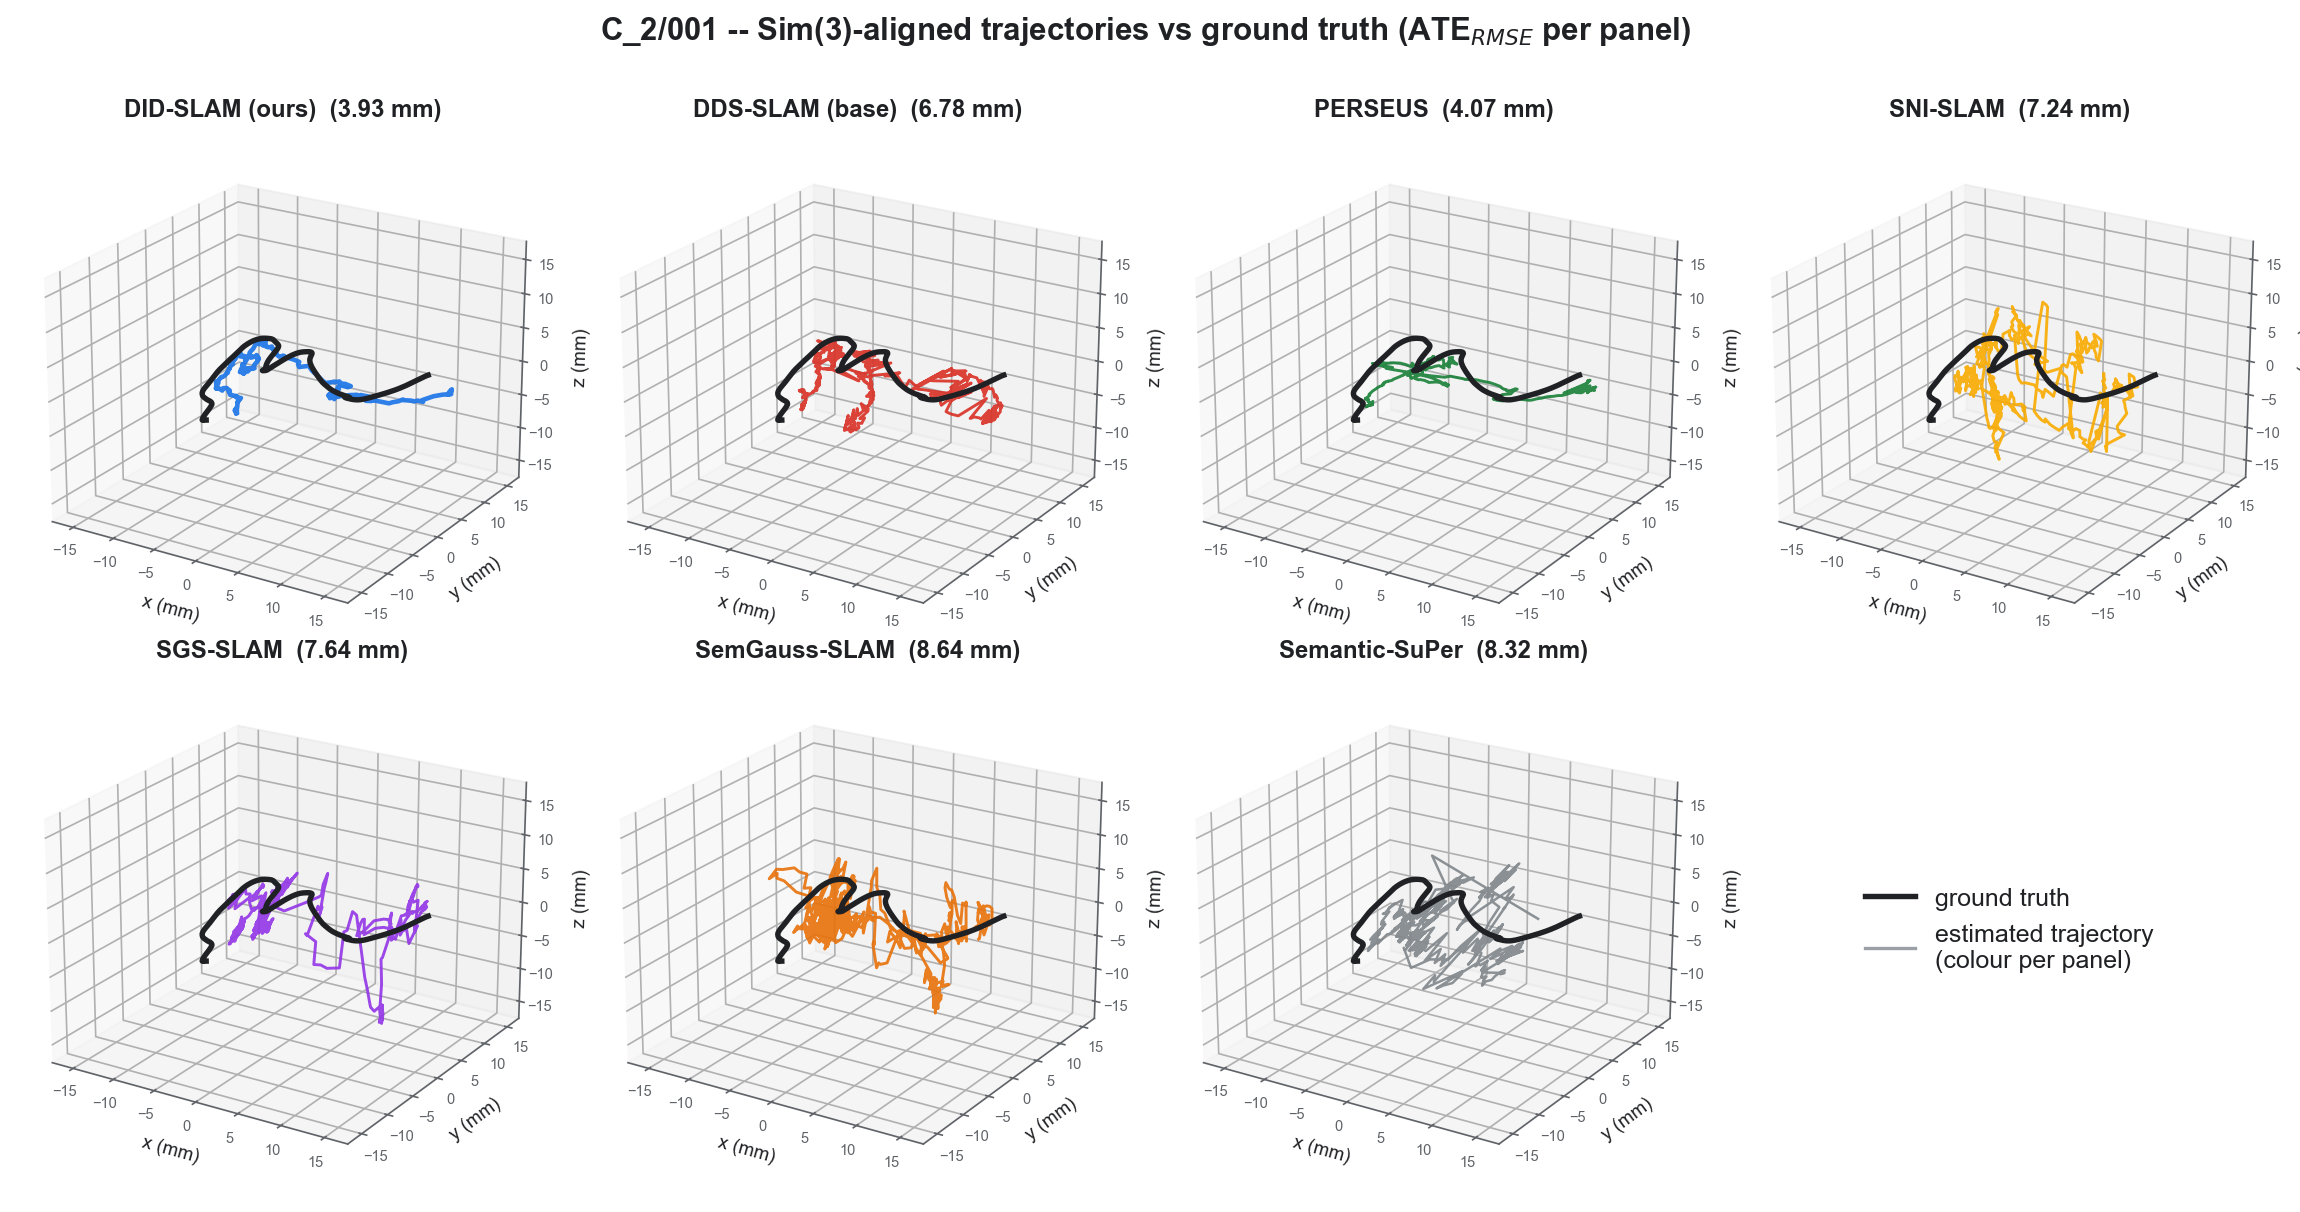
\includegraphics[width=\linewidth]{figures/fig_traj3d_compare.png}
    \caption{Sim(3)-aligned trajectories of every benchmarked system against ground
    truth on C\_2/001. One panel per system (ATE$_{\mathrm{RMSE}}$ in each
    title): DID-SLAM follows the true path; the render-loss trackers oscillate
    around it while under- and over-travelling.}
    \label{fig:traj3d_compare}
\end{figure}

\begin{figure}[!ht]
    \centering
    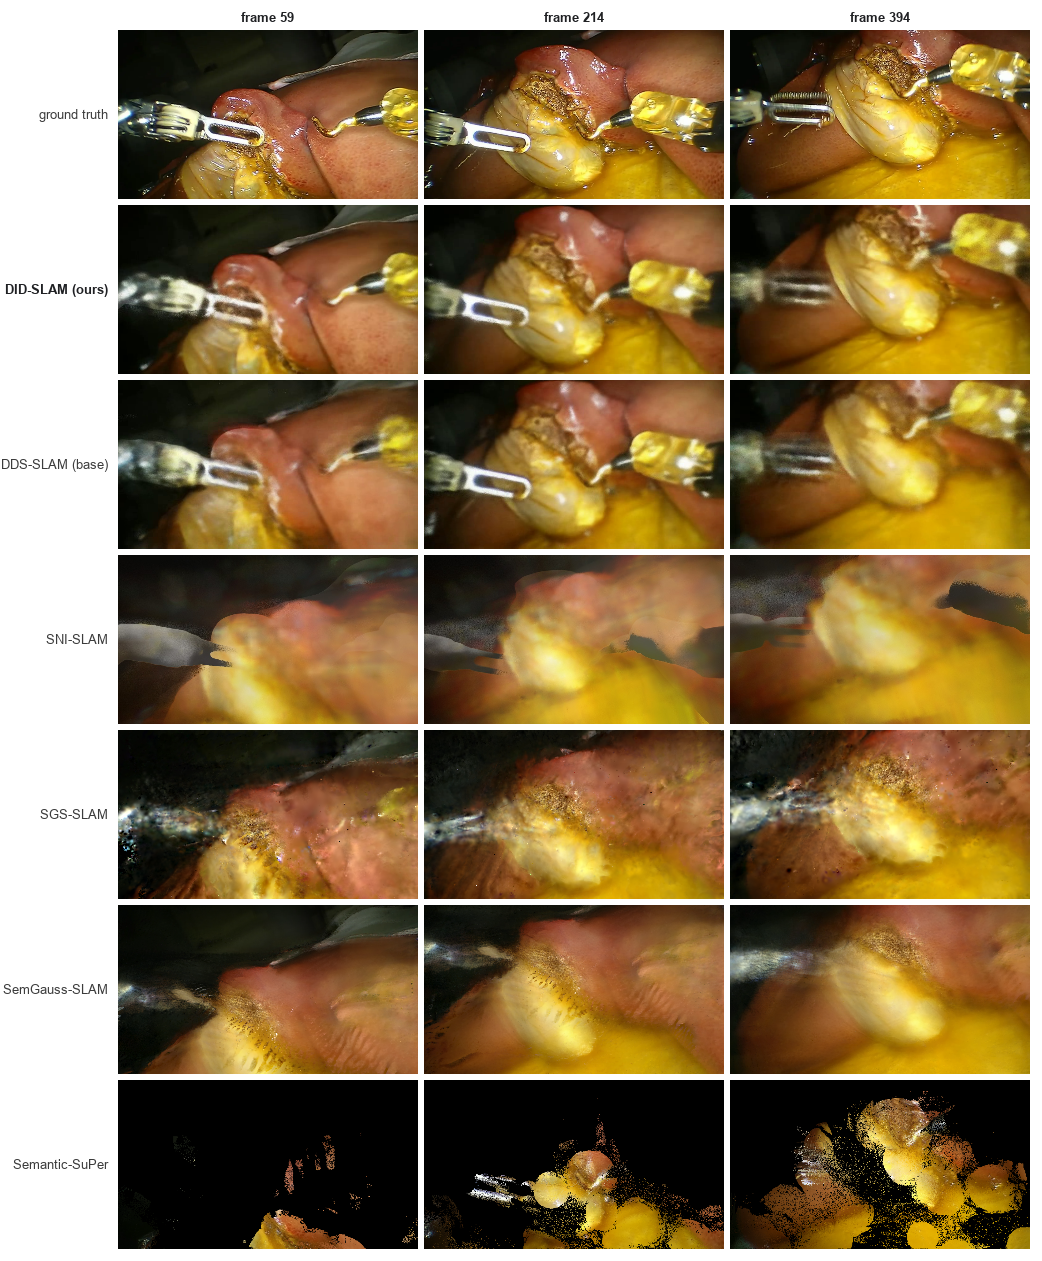
\includegraphics[width=\linewidth]{figures/fig_render_compare.png}
    \caption{Three C\_2/001 frames rendered by every system against the input frame (PERSEUS is tracking-only and renders nothing). Frames are chosen where DID-SLAM's per-frame PSNR exceeds the base's while every system produces a valid render. DID and the base render the sharpest; the other systems degrade as discussed in Section~\ref{sec:discussion}.}
    \label{fig:render_compare}
\end{figure}
\FloatBarrier
\section{Discussion}
\label{sec:discussion}

DID-SLAM's tracking improvements come from three interventions. The motion-attribution gate removes ambiguous frames \emph{outright}: when the evidence says the camera is still, the pose is frozen rather than solved, so no error can enter on that frame at all. The uncertainty head works \emph{within} the frames that are kept, down-weighting the rays --- deforming tissue, moving instruments, specularities --- that the static field cannot explain, so the pose solve leans on the measurements it can trust. Finally, the optimised hyperparameters: lowering the bundle-adjustment pose learning rate to $10^{-5}$ greatly reduces an optimiser-induced noise floor (Section~\ref{sec:hyperparams}) the same size as the true inter-frame motion, which would otherwise corrupt every keyframe regardless of what the model decided.

The clearest pattern in the benchmark is a shared failure regime. CRCD camera motion is small enough that, for long stretches, the true inter-frame motion falls below the optical-flow noise floor, so every system must decide what to do when the image no longer carries motion evidence. The render-loss trackers manufacture it: the base, SNI-SLAM, SGS-SLAM and SemGauss-SLAM over-travel the true path by $3$--$24\times$, oscillating around it as sampling noise and deforming content are absorbed into the pose (Figures~\ref{fig:traj3d_compare} and~\ref{fig:did_traj_c2}). PERSEUS fails the opposite way for the same reason: its motion filter gates sub-threshold flow and stops updating, so on the deforming E\_3/005 its estimate under-travels (path ratio $0.51$). Both behaviours agree that when image motion drops below the noise floor the correct action is not to track; they differ only in whether that decision is deliberate. DID-SLAM makes it explicitly, through the motion-attribution gate, and, unlike PERSEUS's filter, reverses it as soon as motion evidence returns, which keeps the freeze from degenerating into the compact, frozen trajectory that ATE alone would reward. This is why the shape diagnostics are reported throughout: on near-still sequences a compact trajectory and a correct one are indistinguishable by trajectory error, and only the path ratio and aligned correlation separate them.

\begin{figure}[!ht]
    \centering
    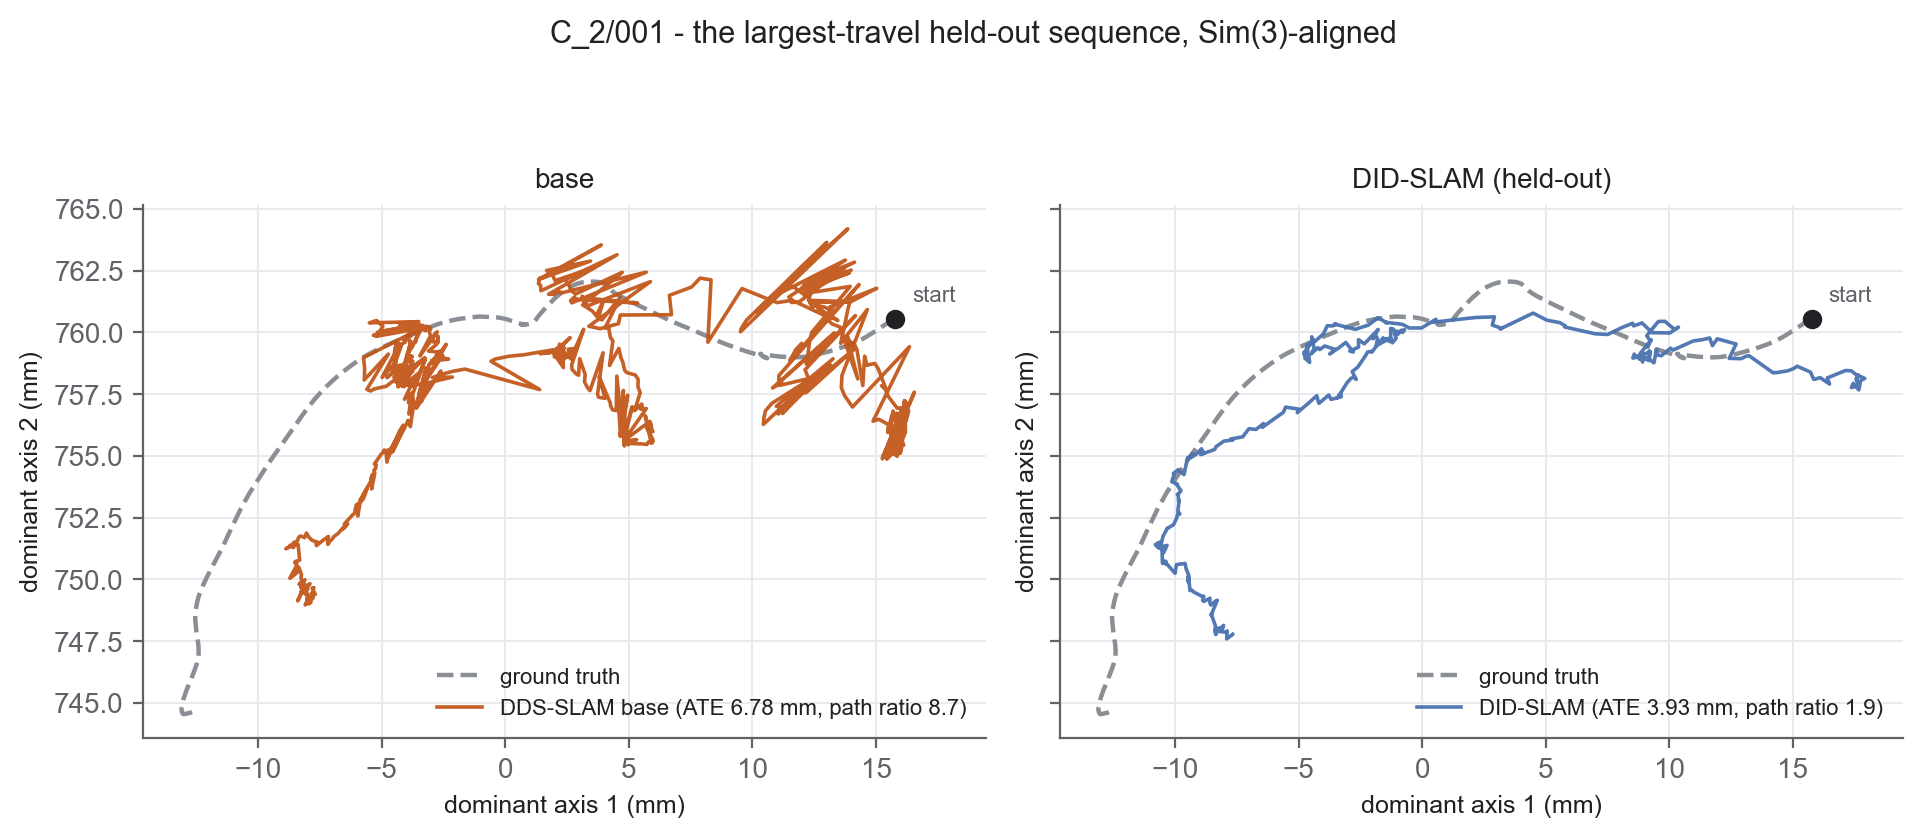
\includegraphics[width=\linewidth]{figures/bdds_traj_c2.png}
    \caption{Estimated trajectory against ground truth on C\_2/001, the largest-travel held-out sequence, both Sim(3)-aligned and shown on the ground-truth dominant plane. The base estimate (left) follows the true path's shape but oscillates violently around it, accumulating $8.7\times$ the true path length; DID-SLAM (right) removes the oscillation ($1.9\times$) and halves the trajectory error, on a sequence it never saw during development.}
    \label{fig:did_traj_c2}
\end{figure}
\FloatBarrier

SGS-SLAM's keyframe renders carry the most high-frequency texture in the benchmark and lead LPIPS on two sequences (Figure~\ref{fig:render_compare}), but its tracking trails DID-SLAM on every sequence: the explicit Gaussian map buys texture at a cost the neural-SDF render avoids, and pays for it in the pose. SemGauss-SLAM exports both halves of the problem and trails on each, and its per-Gaussian semantic feature field sets a memory ceiling that an exploratory endoscopic sequence duly collects; its G\_3/001 run exhausted an A100-80GB at eleven million Gaussians. Semantic-SuPer, which attacks the same scenes from the opposite direction with a static camera and a deformation-first map, produces its closest trajectory on the near-static C\_3/001 and breaks everywhere the static-camera assumption does. The consistent picture is that on deforming scenes supervised by monocular depth, a neural-SDF substrate with explicit motion handling is the stronger platform for the tracking half of the problem, and gives up little on the mapping half to get there: DID-SLAM holds the best SSIM of any method on every sequence, and trails the base on PSNR only because of the Charbonnier photometric loss (Section~\ref{sec:results_main}).

Sequences at the CRCD's motion scale proved challenging for every system onboarded: SemGauss-SLAM could not complete the longest sequence on an 80\,GB GPU, Semantic-SuPer required guarding a crash in its own data association to survive the gallbladder retraction, and the systems that did complete span path ratios from $0.5$ to $33\times$ against the true camera path. This is evidence that the still-dominated, deforming, sub-noise-floor regime these sequences capture is not the one existing systems were built or evaluated in: indoor benchmarks in the Replica style carry metres of confident camera travel over a rigid world, and reward exactly the behaviours that fail here. A benchmark that separates trajectory error from trajectory \emph{character} is therefore a prerequisite for measurable progress on surgical SLAM, and the shape diagnostics of Section~\ref{sec:eval_shape} are as much a part of the contribution as the sequences themselves.

The motion attribution pays on the deforming sequence and the corrected bundle-adjustment configuration on the still one, and the final configuration is a joint selection rather than a collection of per-sequence winners; the lowered dissent threshold produced the best single C\_1/001 of any configuration evaluated and was still rejected, because the same setting was the worst on E\_3/005. The uncertainty head is the exception: it is neutral alone on the design sequences, and its value rests on the held-out transfers rather than the design-set ladder. That neutrality is itself informative. If down-weighting unreliable rays changes little in isolation, then the dominant error on these sequences is not mapping corruption by deforming content but pose over-travel --- optimiser noise and unfrozen still frames --- which is precisely what the gate and the bundle-adjustment fix target directly. The head's contribution stays latent until the weighted solve operates on the moving frames the gate leaves behind. This is stated rather than left implicit: attributing improvement to the component that carries the narrative, rather than the one that carries the measurement, is the failure the flag-gated protocol (Section~\ref{sec:setup}) was designed to prevent.

E\_3/005 improves by $12\%$ over the base yet keeps the weakest shape correlation of the five ($0.46$), and most of its remaining error sits in a segment where the true camera motion falls below the flow noise floor. No threshold on a flow statistic can recover motion the flow cannot see: the gate can decide not to be fooled, but it cannot conjure evidence where the sensor provides none.

Three directions follow from where the system stops. First, the flow noise floor is a property of the sensor, not the scene: the dVRK kinematic stream that supplies our ground-truth trajectory exists intra-operatively in any robotic procedure, and even a coarse kinematic prior on the endoscope would hand the gate motion evidence below the optical floor, turning the hardest failure regime into the most tractable one. Second, a representation with explicit, supervised per-region motion is the natural successor to the render-loss-only warp, letting the map explain the deformation rather than asking the pose solve to survive it. Third, the motion-attribution signal is currently consumed only as a binary gate; preliminary experiments that reuse its egomotion-removed residual to steer the mapping budget --- concentrating optimisation on the most-deforming content --- improved trajectory shape on the deforming sequence without touching the pose solve, and suggest the same signal has more to give on the mapping side.

\paragraph{Limitations.} The quantitative results in this thesis are reported at a single random seed per configuration. The intended protocol --- a mean over repeated seeds, judged against the baseline's seed-to-seed spread --- was applied only where noted (the base on E\_3/005), because the compute to repeat every configuration, sequence and benchmark system was not available within the project; covering the full method and the five-system benchmark at a single seed was prioritised over covering a subset at three. The consequence is stated rather than hidden: the baseline's measured spread on the deforming sequence ($\pm 0.60$\,mm) is of the same order as several of the single-seed differences reported there, so small deltas on E\_3/005 should be read as unresolved, while the held-out improvements, large relative to that spread, carry the weight of the claims. Beyond the seed protocol, the study inherits the limitations of its data: the ex-vivo porcine setting removes the respiratory motion present in vivo, the semantic masks are SAM~3 propagations verified by a single annotator without an inter-annotator agreement measure, and depth is monocular and up-to-scale, anchored by stereo at intervals, so tracking is necessarily evaluated under Sim(3) rather than SE(3) and metric scale is never independently validated.

\paragraph{Runtime.} Neither DID-SLAM nor the base it extends runs at anything approaching frame rate. The two were timed on the same Tesla T4 over the same interval, from staged input to reported metrics: DID-SLAM takes $25.8$--$26.5$\,s per frame against the base's $21.5$--$22.2$\,s, so the two contributions cost $16$--$23\%$ of wall clock on matched hardware. The remainder is inherited rather than introduced; it sits in the per-frame neural-SDF optimisation the substrate performs regardless of what the gate or the uncertainty head decide. In absolute terms DID-SLAM runs at $0.038$\,fps: E\_3/005, $4.8$\,s of video, takes $1$\,h\,$57$\,m, and the five evaluation sequences together take $36$\,hours.

\begin{figure}[!ht]
    \centering
    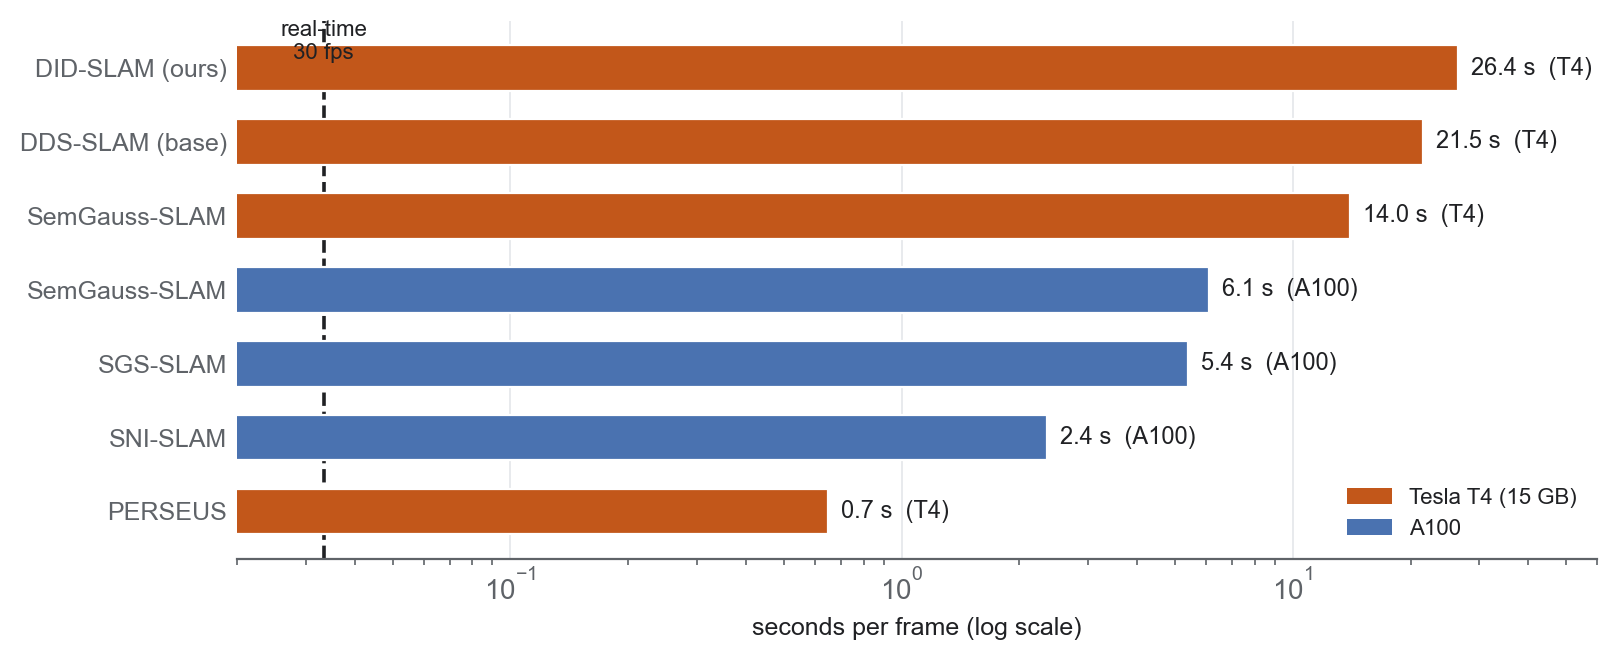
\includegraphics[width=\linewidth]{figures/runtime_bars.png}
    \caption{Per-frame runtime of every benchmarked system, coloured by GPU, against the 30\,fps real-time threshold (dashed). Every system runs one to three orders of magnitude slower than real time. SemGauss-SLAM appears on both a T4 and an A100: the $\sim$2.3$\times$ gap between them is hardware, not method, which is why a cross-system wall-clock column is not tabulated.}
    \label{fig:runtime}
\end{figure}
\FloatBarrier

The Gaussian-splatting systems are markedly quicker (Figure~\ref{fig:runtime}), SGS-SLAM at $5.0$--$5.8$\,s per frame and SemGauss-SLAM at $5.8$--$6.4$\,s, roughly four times faster than our substrate. That comparison is not like-for-like and we do not tabulate it: most of SemGauss-SLAM's runs were executed on an $80$\,GB card while ours ran on a $15$\,GB T4, and the benchmark harnesses did not record device identity at run time, so a wall-clock column would report the hardware at least as much as the method. One accident bounds that confound. SemGauss-SLAM's C\_1/001 run landed on a T4 rather than the $80$\,GB card and took $14.0$\,s per frame against $5.8$--$6.4$\,s on its other snippets, a device factor of roughly $2.3$. Discounting the hardware on that basis still leaves rasterising a Gaussian map cheaper per frame than ray-sampling a signed-distance field, which is a property of the representation rather than of either implementation.

Real-time surgical tracking requires $30$\,fps; DID-SLAM is some $795\times$ short of it, and even the fastest scene-reconstructing system benchmarked here remains well over $100\times$ short. Only PERSEUS approaches interactive rates, at roughly one to two frames per second, and it reaches them by tracking from optical flow while building no map at all, buying speed with the reconstruction half of the problem rather than solving it. Every system that reconstructs the scene therefore sits two to three orders of magnitude away from the regime in which it could inform a surgeon during an operation. A gap that wide does not close by tuning; the plausible route to it is hardware. And the hardware matters: a datacentre A100 is not deployable beside a patient, whereas the T4-class accelerator our timings used is nearer what an embedded surgical system could carry. The numbers reported here are therefore the deployment-relevant ones, not the flattering ones, and the speed-up that would matter arrives as accelerators become faster and more compact, not as this pipeline is better tuned.

\section{Conclusion}
\label{sec:conclusion}
This thesis aimed to narrow two gaps for neural SLAM in surgical environments: the absence of a dataset on which a tracker can be both supervised and honestly evaluated in a deforming scene, and a system that distinguishes camera motion from scene deformation. The reorganised CRCD provides twenty self-contained sequences; dense per-frame semantics from a human-in-the-loop SAM~3 pipeline, stereo-anchored metric depth, and kinematic camera-pose ground truth --- packaged so that existing TUM- and Replica-convention systems load them unmodified; it is, to our knowledge, the only densely-labelled cholecystectomy benchmark against which camera tracking can be evaluated at all. On top of an exactly-reproduced DDS-SLAM base, DID-SLAM adds two flag-gated contributions: a learned aleatoric uncertainty that down-weights the measurements a static field cannot explain, and a label-free motion attribution that separates camera ego-motion from independent scene motion and freezes the pose when the camera is confidently still.

The combination lowers trajectory error on all five evaluation sequences ($-31\%$ on average, $-42\%$ on the largest-travel held-out sequence) while improving SSIM and LPIPS on every one of them, at a cost of $0.6$\,dB of PSNR traceable to the Charbonnier photometric loss, and records the best trajectory of the six benchmarked systems on every sequence. The central finding is that on surgical sequences the true camera motion spends long stretches below the optical-flow noise floor, and every system implicitly decides what to do there: the render-loss trackers manufacture motion, the flow specialist stops updating, and both make that decision by accident. Making that decision explicit, reversible, and attributable to evidence distinguishes DID-SLAM from the systems it was measured against, and the shape diagnostics introduced alongside the benchmark make that difference measurable.

A gate built on optical flow cannot see motion the flow cannot carry, and the dVRK kinematics that supply our ground truth exist intra-operatively in every robotic procedure; a kinematic prior on the endoscope would hand the gate evidence precisely where the optical sensor goes blind. The deformation warp the system inherits is supervised only through the render loss, with no direct motion target; a map that explains deformation, rather than asking the pose solve to survive it, is the natural next platform. And the motion-attribution signal is consumed only as a gate, while preliminary experiments steering the mapping budget with the same signal already improve trajectory shape on the deforming sequence.


\section{Acknowledgments}
\emph{[To be written]}

\bibliographystyle{ieeetr}
\bibliography{references}

\end{document}
